\chapter{Analisis}
\label{chap:analisis}
Pada analisis membahas mengenai deskripsi sistem terkini dan analisis sistem usulan.

\section{Deskripsi Sistem Terkini}
\label{sec:deskripsi_sistem_terkini}
Deskripsi sistem terkini membahas mengenai gambaran umum institusi, jenis-jenis surat akademik yang dikeluarkan oleh pihak TU, prosedur pemesanan surat akademik, prosedur pembuatan surat akademik, prosedur pengambilan surat akademik dan analisis kebutuhan. \\

\subsection{Gambaran Umum Institusi}
\label{sec:gambaran_umum_institusi}
Fakultas Teknologi Informasi dan Sains (FTIS) adalah salah satu fakultas yang terdapat di kampus Universitas Katolik Parahyangan (UNPAR). FTIS dikepalai oleh seorang dekan yang dibantu oleh 3 wakil dekan. FTIS memiliki 3 program studi (prodi) yaitu Prodi Matematika, Fisika dan Teknik Informatika. Setiap prodi dipimpin oleh seorang ketua prodi yang dibantu oleh seorang sekretaris prodi, kecuali Prodi Fisika. Setiap prodi, kecuali Prodi Matematika, memiliki laboratorium yang dikepalai oleh seorang kepala laboratorium. Untuk mengurusi masalah administrasi fakultas, terdapat bagian Tata Usaha (TU) yang terdiri dari sub bagian (subag) tertentu yang mengurusi bidang tertentu.\

Gambar \hyperlink{organigram_fakultas}{3.1} menjelaskan struktur organisasi dari FTIS. Di bawah ini akan dijelaskan  setiap bagian dari struktur organisasi tersebut. Setiap fungsi pada struktur organisasi tersebut memiliki tugas, wewenang, dan tanggung jawab yang berbeda.
\begin{figure}[H]
	\centering
		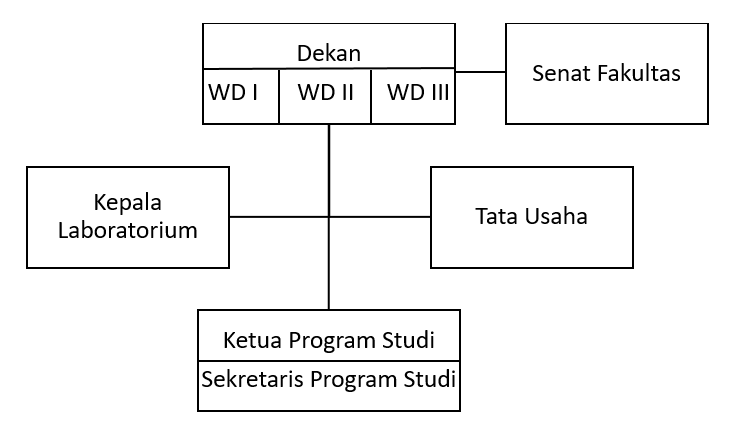
\includegraphics[scale=0.45]{F:/Skripsi/Dokumentasi_Skripsi/Gambar/Diagram/sistem_terkini/organigram/organigram_fakultas_new.PNG}
	\caption{Struktur organisasi Fakultas Teknologi Informasi dan Sains}
	\label{fig:organigram_fakultas}
\end{figure}

\begin{enumerate}
	\item Dekan \\
	berfungsi sebagai pengambil keputusan tertinggi di fakultas.
	\item Senat Fakultas \\
	berfungsi sebagai partner dekan untuk membantu memberikan pertimbangan dari keputusan yang akan diambil. Senat dipilih dari dosen tetap di fakultas.
	\item Wakil Dekan Bidang Akademik (WD I)\\
	berfungsi untuk membantu dekan pada pengambilan segala keputusan yang berhubungan dengan kegiatan akademik yang berlangsung di setiap program studi yang ada pada fakultas.
	\item Wakil Dekan Bidang Sumber Daya (WD II)\\
	berfungsi untuk membantu dekan pada pengambilan segala keputusan yang berhubungan dengan pengelolaan setiap bentuk sumber daya yang terdapat di lingkungan fakultas.
	\item Wakil Dekan Bidang Kemahasiswaan dan Alumni (WD III)\\
	berfungsi untuk membantu dekan pada pengambilan segala keputusan yang berhubungan dengan setiap permasalahan kemahasiswaan dan alumni di lingkungan fakultas.
	\item Kepala Laboratorium \\
	bertanggung jawab akan perawatan dan operasional laboratorium.
	\item Ketua Program Studi \\
	berfungsi sebagai pengambil keputusan tertinggi di lingkungan program studi.
	\item Sekretaris Program Studi \\
	berfungsi untuk membantu ketua program studi pada pengambilan segala keputusan di lingkungan program studi.
	\item Tata Usaha \\
	berfungsi untuk melayani segala kegiatan administrasi yang terjadi di lingkungan FTIS.
\end{enumerate}

Gambar \hyperlink{organigram_TU}{3.2} merupakan struktur organisasi dari TU FTIS. Bagian tata usaha dipimpin oleh seorang Kepala Bagian (Kabag). Di bawah Kabag terdapat 4 sub bagian (Subag) yang dikepalai oleh seorang Kepala Sub Bagian (Kasubag). Berikut ini akan dijelaskan struktur organisasi yang ada di tata usaha FTIS.
\begin{figure}[H]
	\centering
		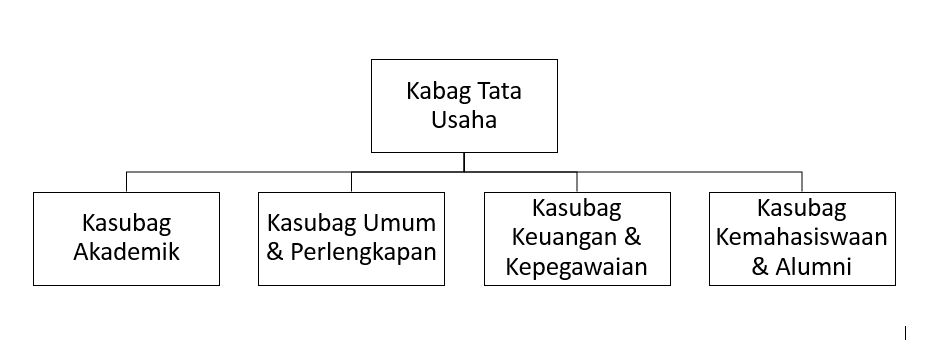
\includegraphics[scale=0.5]{F:/Skripsi/Dokumentasi_Skripsi/Gambar/Diagram/sistem_terkini/organigram/organigram_TU.JPG}
	\caption{Struktur organisasi Tata Usaha Fakultas Teknologi Informasi dan Sains}
	\label{fig:organigram_TU}
\end{figure}
\begin{enumerate}
	\item Kabag Tata Usaha \\
	berfungsi sebagai pemegang keputusan tertinggi di tata usaha.
	\item Kasubag Akademik \\
	berfungsi sebagai pengatur segala hal yang berhubungan dengan kegiatan akademik di lingkungan fakultas, seperti pengaturan jadwal kuliah dan ujian, jadwal perwalian, pembagian ruangan, memperbanyak dan mendistribusikan soal ujian, dll.
	\item Kasubag Umum dan Peralatan \\
	berfungsi sebagai pengatur segala kegiatan, sarana dan prasarana yang ada di lingkungan fakultas. 
	\item Kasubag Keuangan dan Kepegawaian \\
	berfungsi sebagai pengatur operasional keuangan dan kepegawaian di lingkungan fakultas.
	\item Kasubag Kemahasiswaan dan Alumni \\
	berfungsi untuk melayani segala keperluan kemahasiswaan dan alumni seperti keperluan surat menyurat, legalisir ijazah, mempersiapkan perlengkapan wisuda, dll.
\end{enumerate}
Berdasarkan uraian mengenai struktur organisasi fakultas, Kasubag Kemahasiswaan dan Alumni berperan mengurusi keperluan surat menyurat di fakultas. Surat-surat yang dibuat termasuk juga dengan surat akademik yang akan dibahas lebih detil pada subbab selanjutnya.

\subsection{Jenis-Jenis Surat Akademik}
\label{sec:jenis_jenis_surat_akademik}
Ada berbagai macam surat akademik yang dikeluarkan oleh TU FTIS. Surat yang dikeluarkan antara lain sebagai berikut :
\begin{enumerate}
	\item Surat keterangan beasiswa \\
	Surat ini berfungsi sebagai surat pernyataan bahwa mahasiswa yang bersangkutan telah menerima beasiswa dari pihak non-Unpar dan tidak menerima beasiswa lain yang berasal dari Unpar.

	\item Surat keterangan \\
	Surat ini memiliki fungsi yang beragam. Surat ini dapat digunakan untuk pernyataan mahasiswa aktif, pembuatan surat kelakuan baik, membuka rekening, membuat visa, dll.
	
	\item Surat izin studi lapangan \\
	Surat ini berfungsi sebagai surat pengantar apabila ada mahasiswa yang hendak melakukan wawancara, survei, studi banding atau observasi ke sebuah instansi.
	
	\item Surat izin cuti studi \\
	Surat ini berlaku apabila mahasiswa yang bersangkutan tidak akan mengikuti perkuliahan pada semester tertentu. Biasanya surat ini digunakan apabila mahasiswa mengalami sakit keras dan membutuhkan masa penyembuhan yang lama ataupun tidak ada mata kuliah yang dibuka pada semester yang berjalan. Surat ini dapat diproses apabila mahasiswa pemohon telah memenuhi 2 syarat, yaitu tidak memiliki tunggakan pembayaran uang kuliah dan sudah membayar uang cuti studi.
	
	\item Surat izin pengunduran diri mahasiswa \\
	Surat ini berfungsi sebagai surat pernyataan apabila seorang mahasiswa hendak mengundurkan diri dari Unpar. Biasanya lasan pengambilan surat ini dikarenakan mahasiswa yang bersangkutan merasa tidak cocok dengan jurusan atau telah diterima di universitas lain dan hendak berkuliah di universitas tersebut.

	\item Surat perwakilan perwalian \\
	Surat ini berlaku apabila mahasiswa yang bersangkutan berhalangan hadir untuk melakukan perwalian dengan dosen wali sehingga diwakilkan kepada mahasiswa lain yang diberi kuasa.
	
	\item Surat dispensasi pembayaran \\
	Surat ini berlaku apabila mahasiswa yang bersangkutan berencana mengambil mata kuliah kurang dari 10 SKS pada semester yang akan ditempuh. Surat ini harus diproses sebelum masa FRS berlangsung. Surat ini berbentuk formulir isian. Pertama mahasiswa harus mengisi formulir. Setelah formulir diisi sesuai dengan data yang dibutuhkan, formulir akan diteruskan kepada dosen wali dari mahasiswa yang bersangkutan melalui Petugas TU untuk mendapatkan tanda tangan dosen wali. Setelah mendapat tanda tangan dosen wali, formulir diteruskan kepada Biro Keuangan Unpar untuk mendapatkan persetujuan. Apabila disetujui, akan dikirimkan surat persetujuan kepada Petugas TU untuk mengubah jumlah tagihan pembayaran uang kuliah milik mahasiswa di situs \textit{studentportal}. Sehingga jumlah tagihan yang muncul akan sesuai dengan SKS mata kuliah yang akan diambil. 
	
	\item Surat pengajuan pengambilan kelebihan pembayaran uang kuliah (tunai) \\
	Surat ini berlaku apabila mahasiswa yang bersangkutan telah membayar uang kuliah sesuai dengan SKS mata kuliah yang diambil namun kemudian membatalkan mata kuliah yang telah diambil tersebut. Surat ini berbentuk formulir isian. Pertama mahasiswa harus mengisi formulir. Setelah formulir diisi sesuai dengan data yang dibutuhkan, formulir akan ditandatangani oleh Petugas TU. Setelah ditandatangani, formulir diteruskan kepada Biro Keuangan Unpar untuk diproses. Setelah diproses akan dikirimkan surat keterangan pengembalian uang kuliah beserta sejumlah uang kelebihan pembayaran kuliah kepada Petugas TU. Uang akan diberikan kepada mahasiswa pemohon dan surat keterangan akan disimpan di TU sebagai arsip.

	\item Surat penundaan pembayaran uang kuliah \\
	Surat ini berlaku apabila mahasiswa yang bersangkutan belum bisa membayar uang kuliah sampai tanggal yang telah ditentukan. Fungsi surat ini yaitu untuk memberikan kelonggaran waktu pembayaran uang kuliah pada mahasiswa sehingga mahasiswa yang bersangkutan akan terlepas dari denda keterlambatan pembayaran. Pertama mahasiswa harus mengisi formulir. Setelah formulir diisi sesuai dengan data yang dibutuhkan, akan dibuatkan surat yang kemudian diteruskan kepada Wakil Dekan Bidang Sumber Daya melalui Petugas TU untuk mendapatkan tanda tangan wakil dekan. Setelah mendapat tanda tangan wakil dekan, surat diteruskan kepada Biro Keuangan Unpar untuk mendapatkan persetujuan. Apabila disetujui, akan dikirimkan surat persetujuan kepada Petugas TU yang menyatakan pemberian izin kepada mahasiswa pemohon untuk menunda pembayaran uang kuliah.
	
	\item Surat permohonan beasiswa \\
	Surat ini berfungsi apabila seorang mahasiswa hendak mengajukan beasiswa kepada universitas maupun fakultas. Surat ini berbentuk formulir isian. Setelah formulir diisi sesuai dengan data yang dibutuhkan, formulir diteruskan kepada dosen wali mahasiswa pemohon untuk mendapat catatan dan tanda tangan dosen wali. Setelah itu surat akan diteruskan kepada dekan untuk catatan dan tanda tangan dekan. Setelah semua data terisi lengkap, formulir akan diserahkan kepada Badan Kemahasiswaan dan Alumni Unpar.
	\end{enumerate}

\subsection{Prosedur Pemesanan Surat}
\label{sec:prosedur_pemesanan_surat}
Gambar \hyperlink{pemesanan_terkini}{3.3} merupakan prosedur pemesanan surat yang dilakukan oleh mahasiswa kepada Kasubag Kemahasiswaan dan Alumni. Untuk selanjutnya Kasubag Kemahasiswaan dan Alumni akan disebut sebagai Petugas TU untuk mempersingkat penyebutan nama. Prosedur pemesanan surat dimulai dengan:
\begin{enumerate}
	\item Mahasiswa mendatangi Petugas TU dan menyebutkan surat yang dibutuhkan
	\item Petugas TU memberikan formulir yang harus diisi sesuai dengan surat yang dibutuhkan
	\item Mahasiswa mengisi formulir
	\item Mahasiswa mengembalikan formulir ke Petugas TU
	\item Petugas TU mengecek pengisian formulir. Apabila ada kesalahan pengisian, maka formulir dikembalikan kepada mahasiswa untuk diperbaiki. Jika tidak ada kesalahan maka dapat lanjut ke proses berikutnya
	\item Apabila sedang tidak ada pesanan surat, surat dapat langsung dibuatkan, apabila ada pesanan, surat akan masuk \textit{waiting list} dan Petugas TU akan memberikan estimasi waktu selesai pengerjaan surat
\end{enumerate}

\begin{figure}[H]
	\centering
		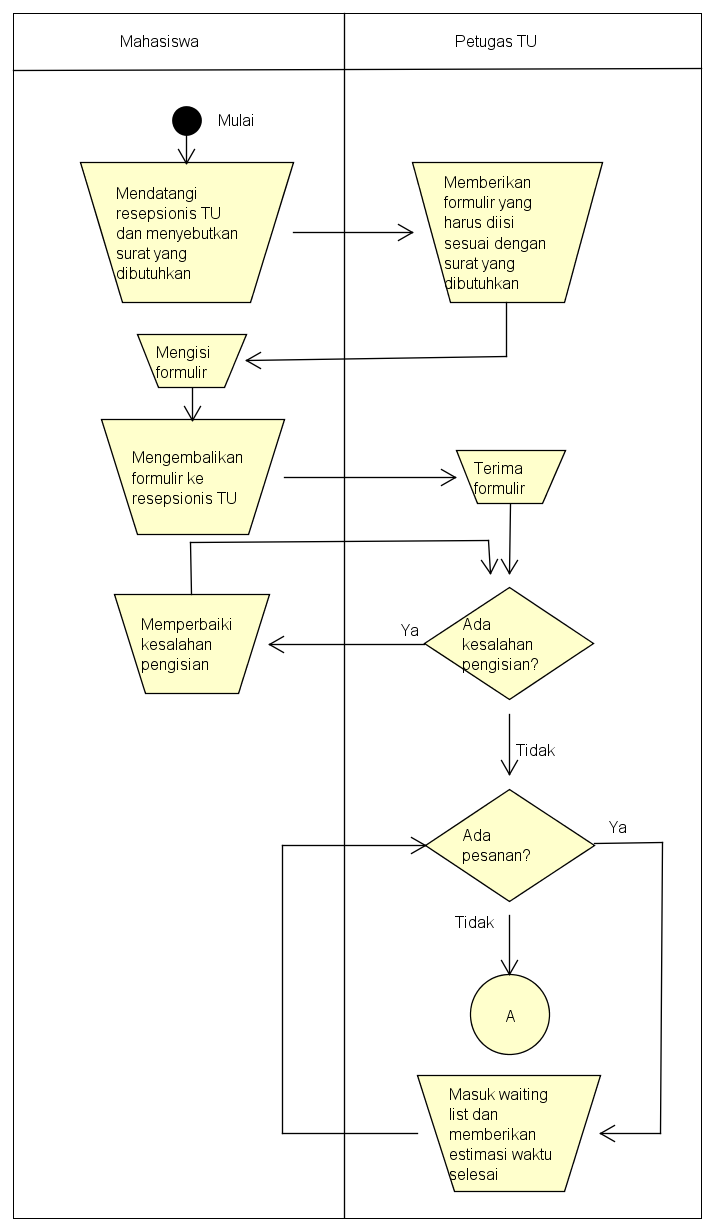
\includegraphics[scale=0.7]{F:/Skripsi/Dokumentasi_Skripsi/Gambar/Diagram/sistem_terkini/work_flow/pemesanan_terkini.png}
	{\caption{Prosedur pemesanan surat terkini}}
	\label{fig:pemesanan_terkini}
\end{figure}

\subsection{Prosedur Pembuatan Surat}
\label{sec:prosedur_pembuatan_surat}
Gambar \hyperlink{pembuatan_terkini}{3.4} merupakan prosedur pembuatan surat yang dilakukan oleh Petugas TU. Prosedur pembuatan surat dimulai dengan:
\begin{enumerate}
	\item Petugas TU mengecek formulir yang telah diisi oleh mahasiswa
	\item Petugas TU membuka \textit{template} surat yang dipesan
	\item Petugas TU memasukkan semua data yang telah dituliskan oleh mahasiswa pada formulir ke \textit{template}
	\item Petugas TU melakukan cek ulang apabila terjadi kesalahan dalam memasukkan data
	\item Apabila tidak ada kesalahan Petugas TU dapat langsung mencetak surat
	\item Petugas akan menghubungi pejabat tertentu yang memiliki keterkaitan dengan surat yang sedang diproses untuk mendapatkan tanda tangan dari pejabat yang bersangkutan
	\item Apabila mahasiswa pemohon menunggu di sekitar ruang TU maka surat dapat langsung diambil oleh mahasiswa pemohon. Apabila tidak ada, maka surat akan disimpan oleh Petugas TU
\end{enumerate}

\begin{figure}[H]
	\centering
		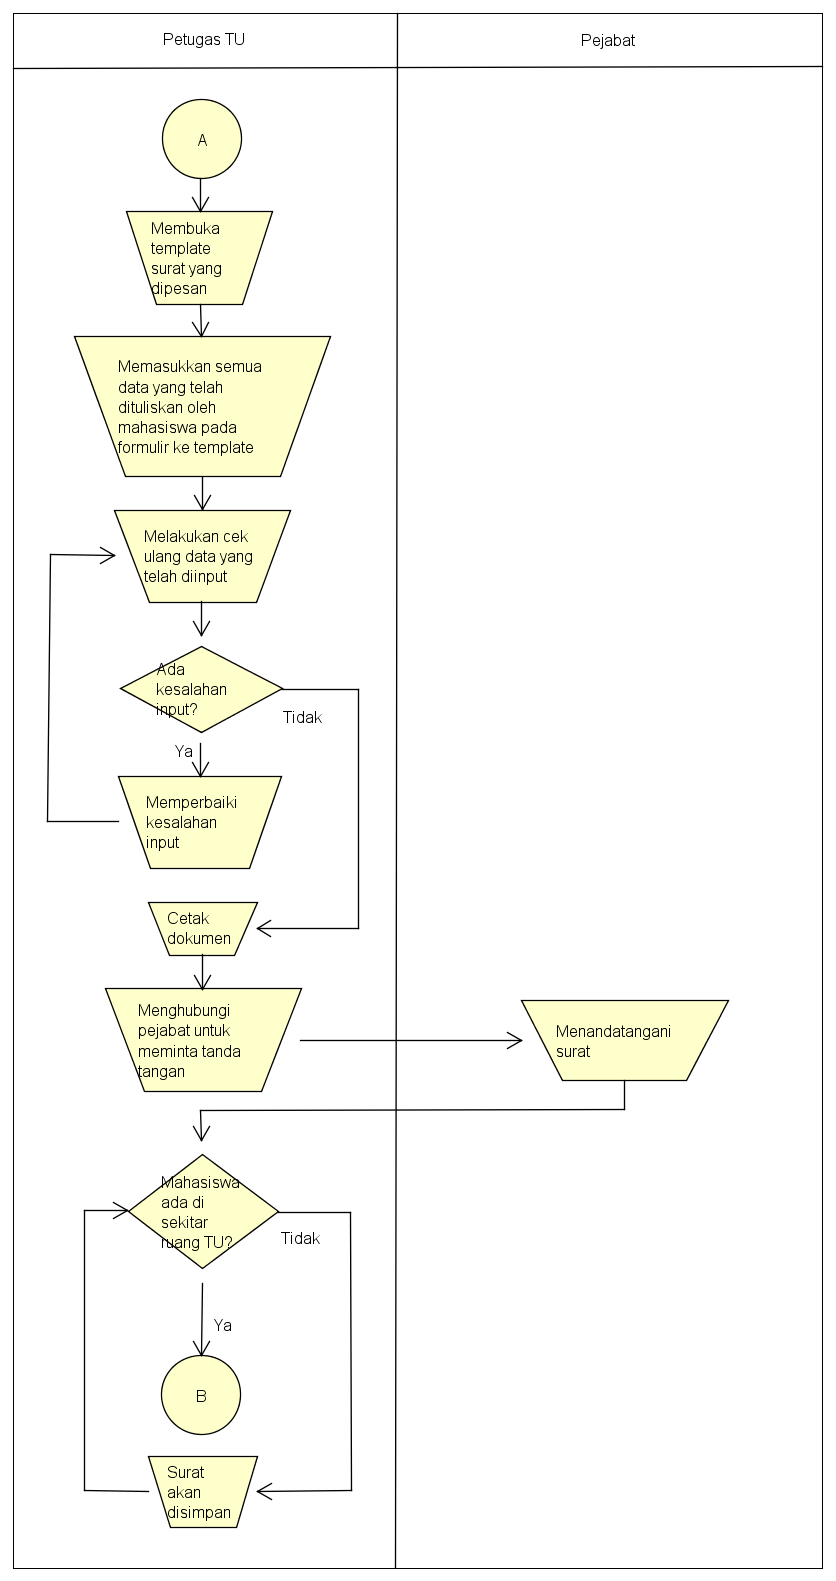
\includegraphics[scale=0.6]{F:/Skripsi/Dokumentasi_Skripsi/Gambar/Diagram/sistem_terkini/work_flow/pembuatan_terkini.png}
	{\caption{Prosedur pembuatan surat terkini}}
	\label{fig:pembuatan_terkini}
\end{figure}

\subsection{Prosedur Pengambilan Surat}
\label{sec:prosedur_pengambilan_surat}
Gambar \hyperlink{pengambilan_terkini}{3.5} merupakan prosedur pengambilan surat yang dilakukan oleh mahasiswa kepada Petugas TU. Prosedur pengambilan surat dimulai dengan:
\begin{enumerate}
	\item Mahasiswa yang memesan mendatangi Petugas TU dan menyebutkan surat apa yang telah dipesan
	\item Petugas TU memberikan surat yang telah dicetak kepada mahasiswa
\end{enumerate}

\begin{figure}[H]
	\centering
		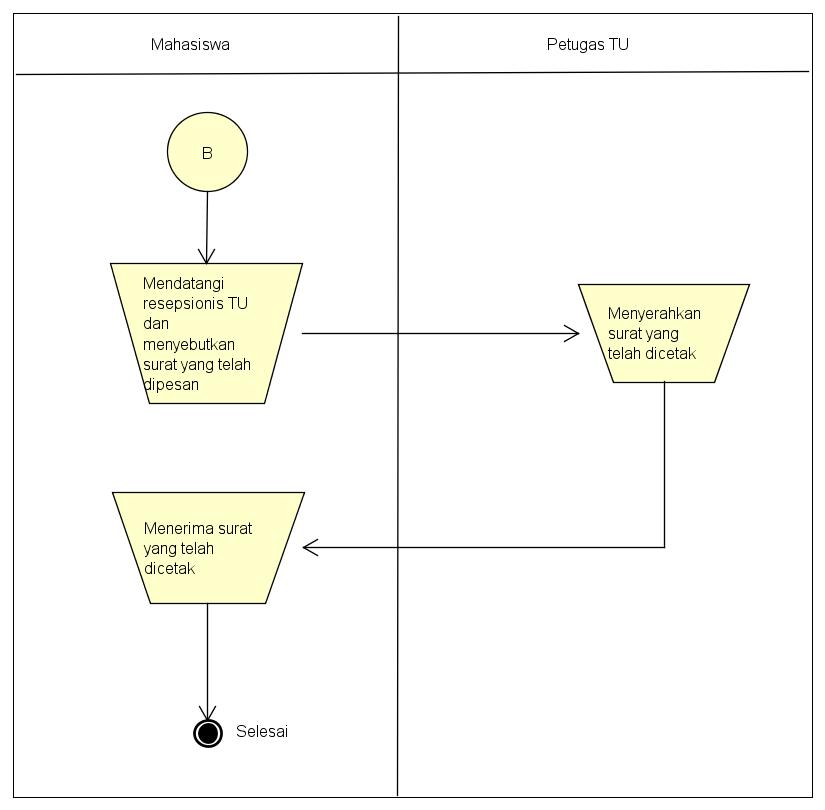
\includegraphics[scale=0.5]{F:/Skripsi/Dokumentasi_Skripsi/Gambar/Diagram/sistem_terkini/work_flow/pengambilan_terkini.jpg}
	{\caption{Prosedur pengambilan surat terkini}}
	\label{fig:pengambilan_terkini}
\end{figure}

\subsection{Analisis Kebutuhan}
\label{sec:analisis_kebutuhan}
Berdasarkan paparan yang telah disebutkan di atas, maka ditemukan beberapa masalah yang menjadi fokus utama dari penelitian ini. Masalah-masalah yang telah ditemukan antara lain:
\begin{enumerate}
	\item Pemesanan surat akademik tidak bisa dilakukan mendadak.
	\item Petugas bisa kewalahan apabila permintaan surat yang masuk cukup banyak dalam sehari.
	\item Ada kemungkinan kesalahan pemasukan data dari formulir ke komputer.
\end{enumerate}

\section{Analisis Sistem Usulan}
\label{sec:analisis_sistem_usulan}
Analisis sistem usulan membahas mengenai surat-surat yang ditangani, prosedur pembuatan surat usulan, \textit{Data Flow Diagram} (DFD), analisis kebutuhan data surat, dan diagram ER. \\

\subsection{Surat-surat yang Ditangani}
\label{sec:surat_yang_ditangani}
Dari 10 surat yang telah disebutkan di atas, diambil 6 surat yang akan dibahas lebih lanjut pada penelitian ini. Hal ini dikarenakan 6 surat tersebut dapat menghasilkan surat yang kemudian akan dikembalikan kepada mahasiswa yang bersangkutan untuk kemudian disampaikan kepada lembaga yang membutuhkan surat tersebut. Dari keenam surat tersebut ada satu surat yang memiliki fungsi ganda yaitu surat keterangan sehingga dibuat menjadi 2 jenis surat yang berbeda sehingga total terdapat 7 surat yang akan dibahas. Ketujuh surat tersebut yaitu :
\begin{enumerate}
	\item Surat keterangan beasiswa \\
	Surat pernyataan bahwa mahasiswa ybs. tidak menerima beasiswa dari pihak universitas maupun fakultas dan hanya menerima beasiswa dari satu organisasi/perusahaan saja.
	\item Surat keterangan mahasiswa aktif \\
	Surat pernyataan bahwa mahasiswa ybs. merupakan mahasiswa aktif Fakultas Teknologi Informasi dan Sains Uiversitas Katolik Parahyangan.
	\item Surat pengantar pembuatan visa \\
	Surat yang pengantar yang diajukan mahasiswa kepada suatu kedutaan besar negara asing dengan tujuan untuk untuk membuat visa.
	\item Surat izin studi lapangan \\
	Surat izin yang diajukan apabila seorang mahasiswa hendak melakukan penelitian ke suatu organisasi dan membutuhkan surat pengantar dari fakultas sebagai syarat penelitian. Surat ini dapat digunakan untuk perorangan maupun kelompok. Untuk surat izin studi lapangan kelompok, dapat mewakili 1 orang ketua dan maksimal 4 orang anggota.
	\item Surat perwalian yang diwakilkan \\
	Surat yang diajukan oleh mahasiswa apabila mahasiswa ybs. berhalangan hadir pada saat perwalian dan hendak diwakilkan oleh mahasiswa lain. 
	\item Surat izin cuti studi \\
	Surat yang diajukan oleh mahasiswa apabila mahasiswa ybs. hendak mengambil cuti studi pada semester tertentu. Surat ini memerlukan lampiran dari orang tua/wali untuk
	\item Surat izin pengunduran diri mahasiswa \\
	Surat yang diajukan oleh mahasiswa apabila mahasiswa ybs. hendak mengundurkan diri dari Fakultas Teknologi Informasi dan Sains Universitas Katolik Parahyangan.
\end{enumerate}

\subsection{Prosedur Pembuatan Surat Usulan}
\label{sec:pembuatan_surat_usulan}
Gambar \hyperlink{pembuatan_usulan}{3.6} merupakan prosedur pembuatan surat yang dilakukan oleh mahasiswa. Pada prosedur usulan ini, untuk membuat surat akademik tidak perlu melalui 3 tahapan seperti yang dijelaskan pada subbagian sistem terkini. Prosedur pembuatan surat dimulai dengan:
\begin{enumerate}
	\item Mahasiswa melakukan login
	\item Mahasiswa memilih kategori surat yang akan dibuat
	\item Mahasiswa memilih jenis surat yang akan dibuat
	\item Mahasiswa memasukkan data yang dibutuhkan dengan benar
	\item Mahasiswa menekan tombol \textit{preview} untuk melihat surat secara keseluruhan
	\item Apabila terdapat kesalahan pada pengisian data, mahasiswa dapat mengklik tombol "Kembali" untuk memperbaiki kesalahan pada pengisian data.
	\item Apabila tidak ada kesalahan, mahasiswa dapat menekan tombol "Buat Surat" untuk memesan surat tersebut dan surat akan masuk ke \textit{database} pesanan surat.
	\item Apabila \textit{id} surat adalah 9 atau 10, surat perlu melalui tahap persetujuan dari Pejabat. Sedangkan surat dengan \textit{id} 1-9 atau 11-20 maka surat dapat langsung diberi nomor surat.
	\item Setelah surat diberi nomor surat, surat dapat di-\textit{generate} menjadi \textit{file} PDF dan surat siap untuk dicetak.	
	\item Setelah surat dicetak, surat akan ditandatangani oleh Pejabat yang berwenang menandatangani surat tersebut. Apabila surat sudah ditandatangani, Pejabat akan mengubah status penandatanganan surat dari "Belum" menjadi "Sudah".
	\item Setelah surat ditandatangani, Petugas TU mengembalikan surat yang sudah ditanda tangani tersebut kepada mahasiswa. Apabila surat sudah diambil oleh mahasiswa pemohon, Petugas TU akan mengubah status pengambilan surat dari "Belum" menjadi "Sudah".
	\
\end{enumerate}
\begin{figure}[H]
	\centering
		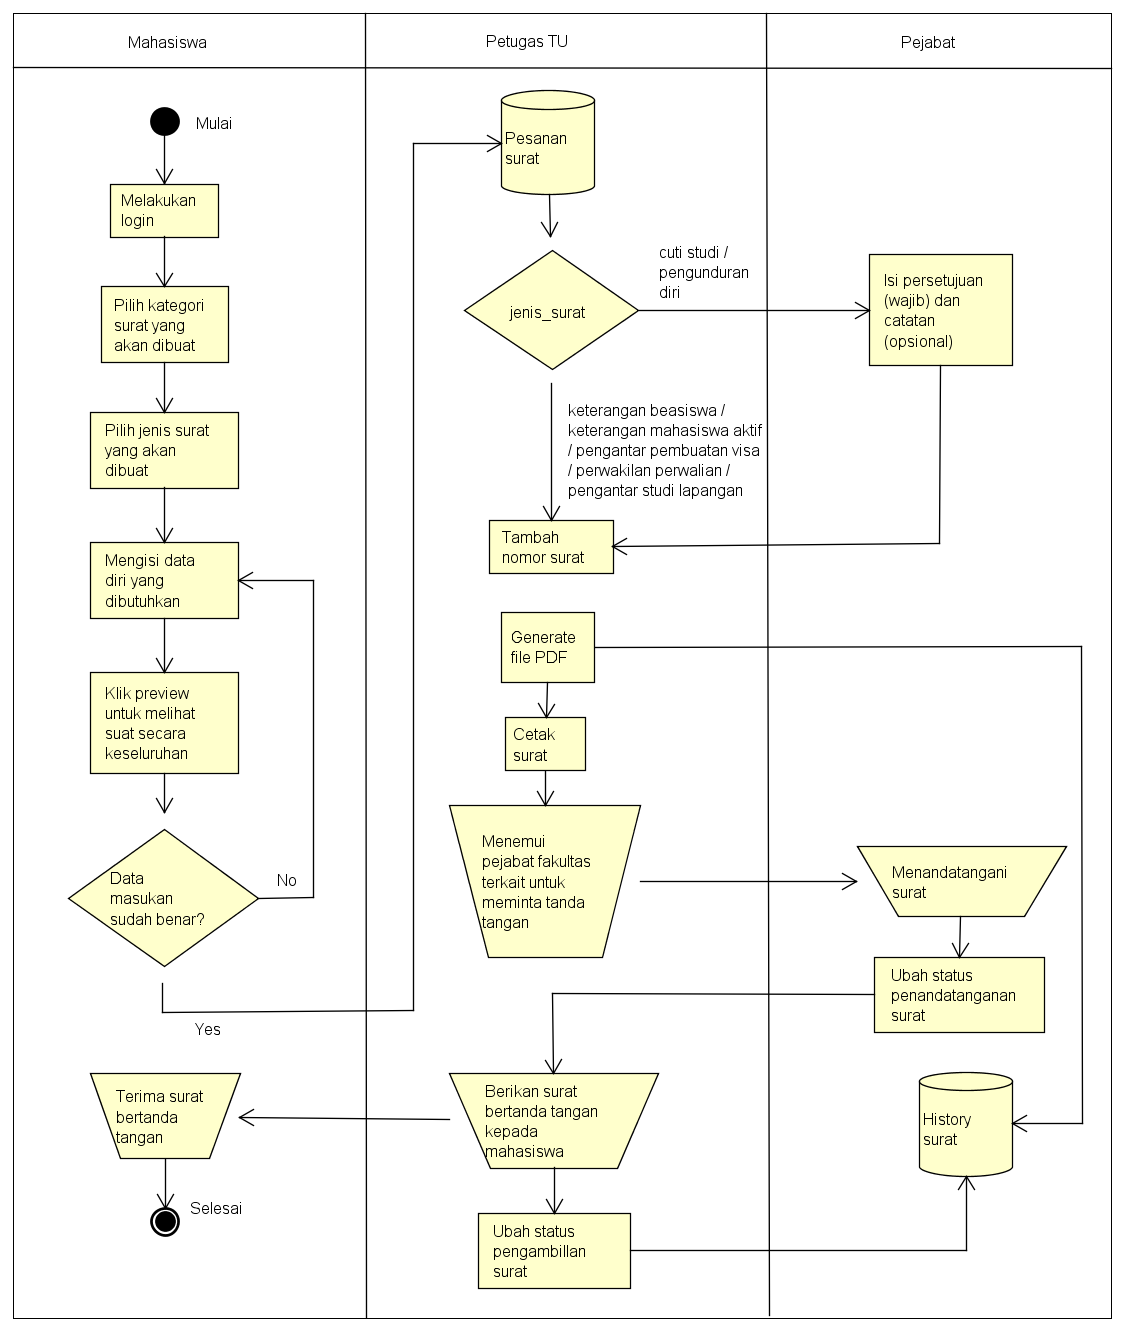
\includegraphics[scale = 0.5]{F:/Skripsi/Dokumentasi_Skripsi/Gambar/Diagram/sistem_usulan/flowchart/Flowchartsmaller.png}
	{\caption{Prosedur pembuatan surat usulan}}
	\label{fig:pembuatan_usulan}
\end{figure}

\subsection{\textit{Data Flow Diagram (DFD)}}
\label{sec:data_flow_diagram}
\textit{Data Flow Diagram (DFD)} adalah diagram untuk memodelkan setiap aliran data pada sistem yang akan dibangun.
Gambar \hyperlink{data_flow}{3.7} merupakan diagram \textit{context} atau DFD \textit{level} 0 yang menjelaskan 
keseluruhan sistem beserta aktornya.

\begin{figure}[H]
	\centering
		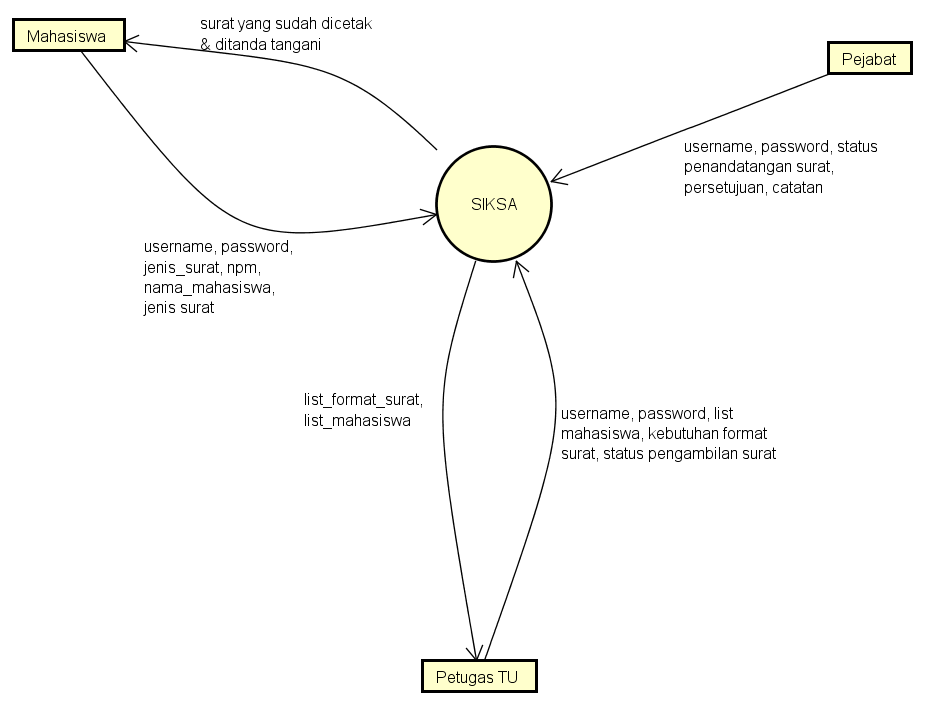
\includegraphics[scale = 0.6]{F:/Skripsi/Dokumentasi_Skripsi/Gambar/Diagram/sistem_usulan/dfd/Lv0.png}
	\caption{Diagram \textit{context}}
	\label{fig:data_flow}
\end{figure}

\textit{Website} penyedia surat akademik ini memiliki 3 aktor, yaitu \textit{mahasiswa}, \textit{pejabat} dan \textit{petugas TU}. Tiap aktor memiliki hak akses ke beberapa fitur tertentu. Gambar \hyperlink{level_1}{3.8} merupakan DFD \textit{level} 1 yang menjelaskan aliran data pada tiap aktor.

\begin{figure}[H]
	\centering
		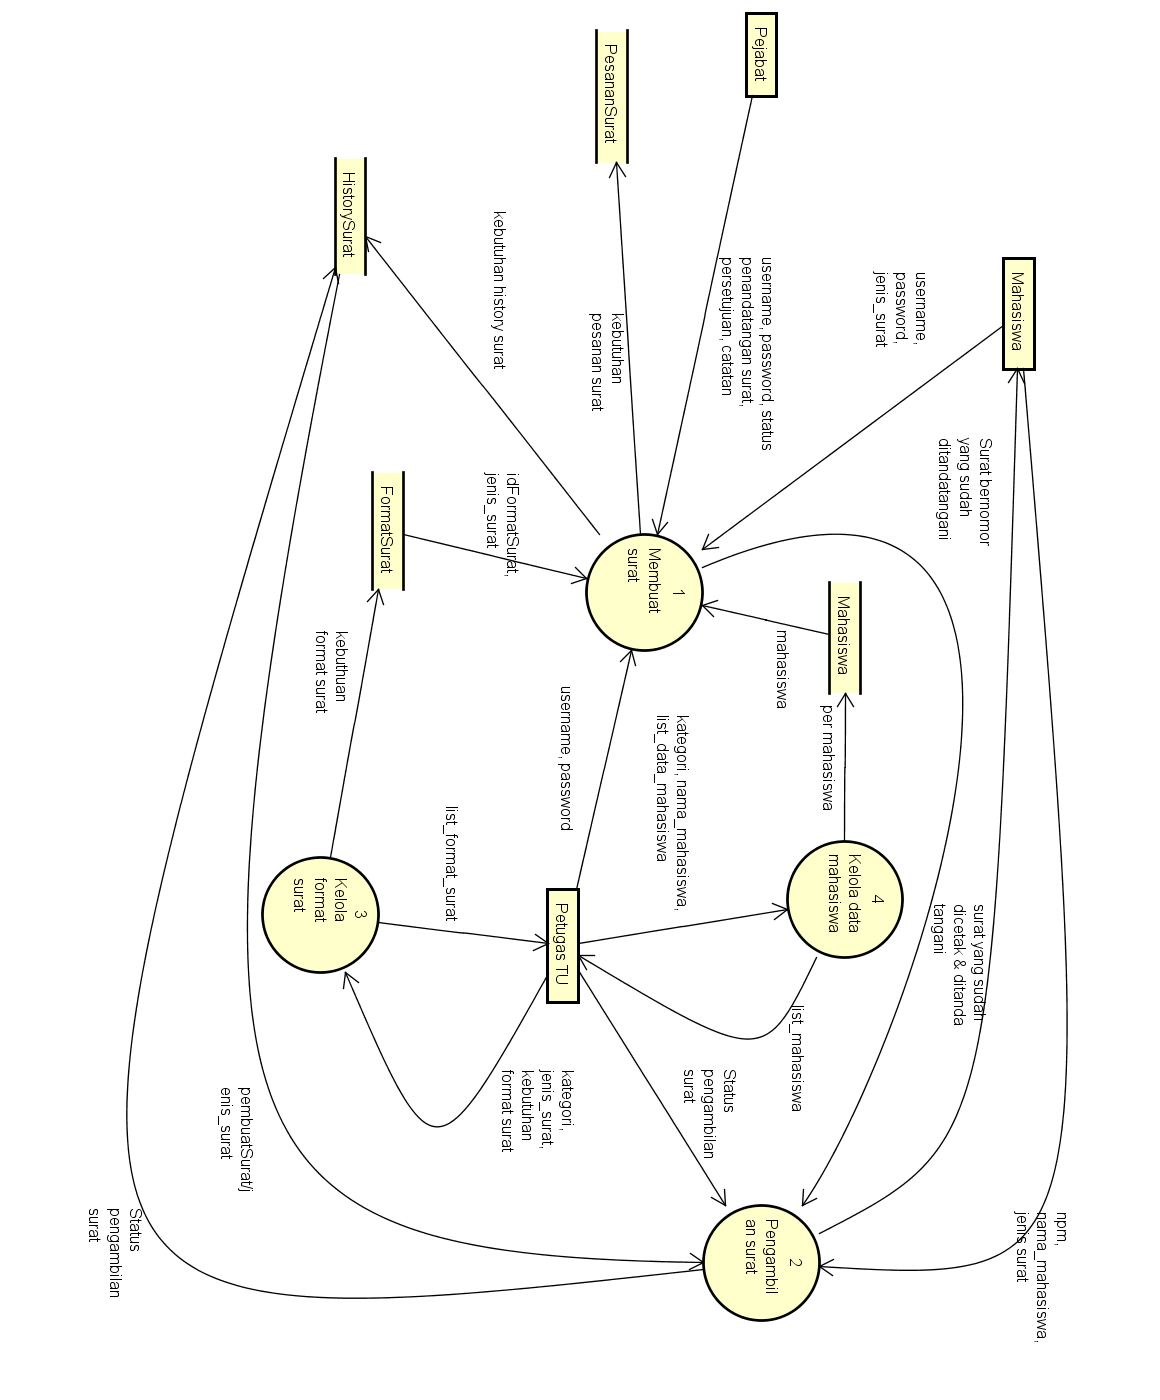
\includegraphics[scale = 0.5]{F:/Skripsi/Dokumentasi_Skripsi/Gambar/Diagram/sistem_usulan/dfd/Lv1-kiri.png}
	\caption{DFD \textit{level} 1}
	\label{fig:level_1}
\end{figure}

Gambar \hyperlink{level_2-1}{3.9} merupakan DFD \textit{level} 2-1 yang menjelaskan aliran data pada saat aktor mahasiswa hendak membuat surat yang kemudian dilanjutkan pada DFD \textit{level} 3-1.10 pada gambar \hyperlink{level_3-1.10}{3.10}

\begin{figure}[H]
	\centering
		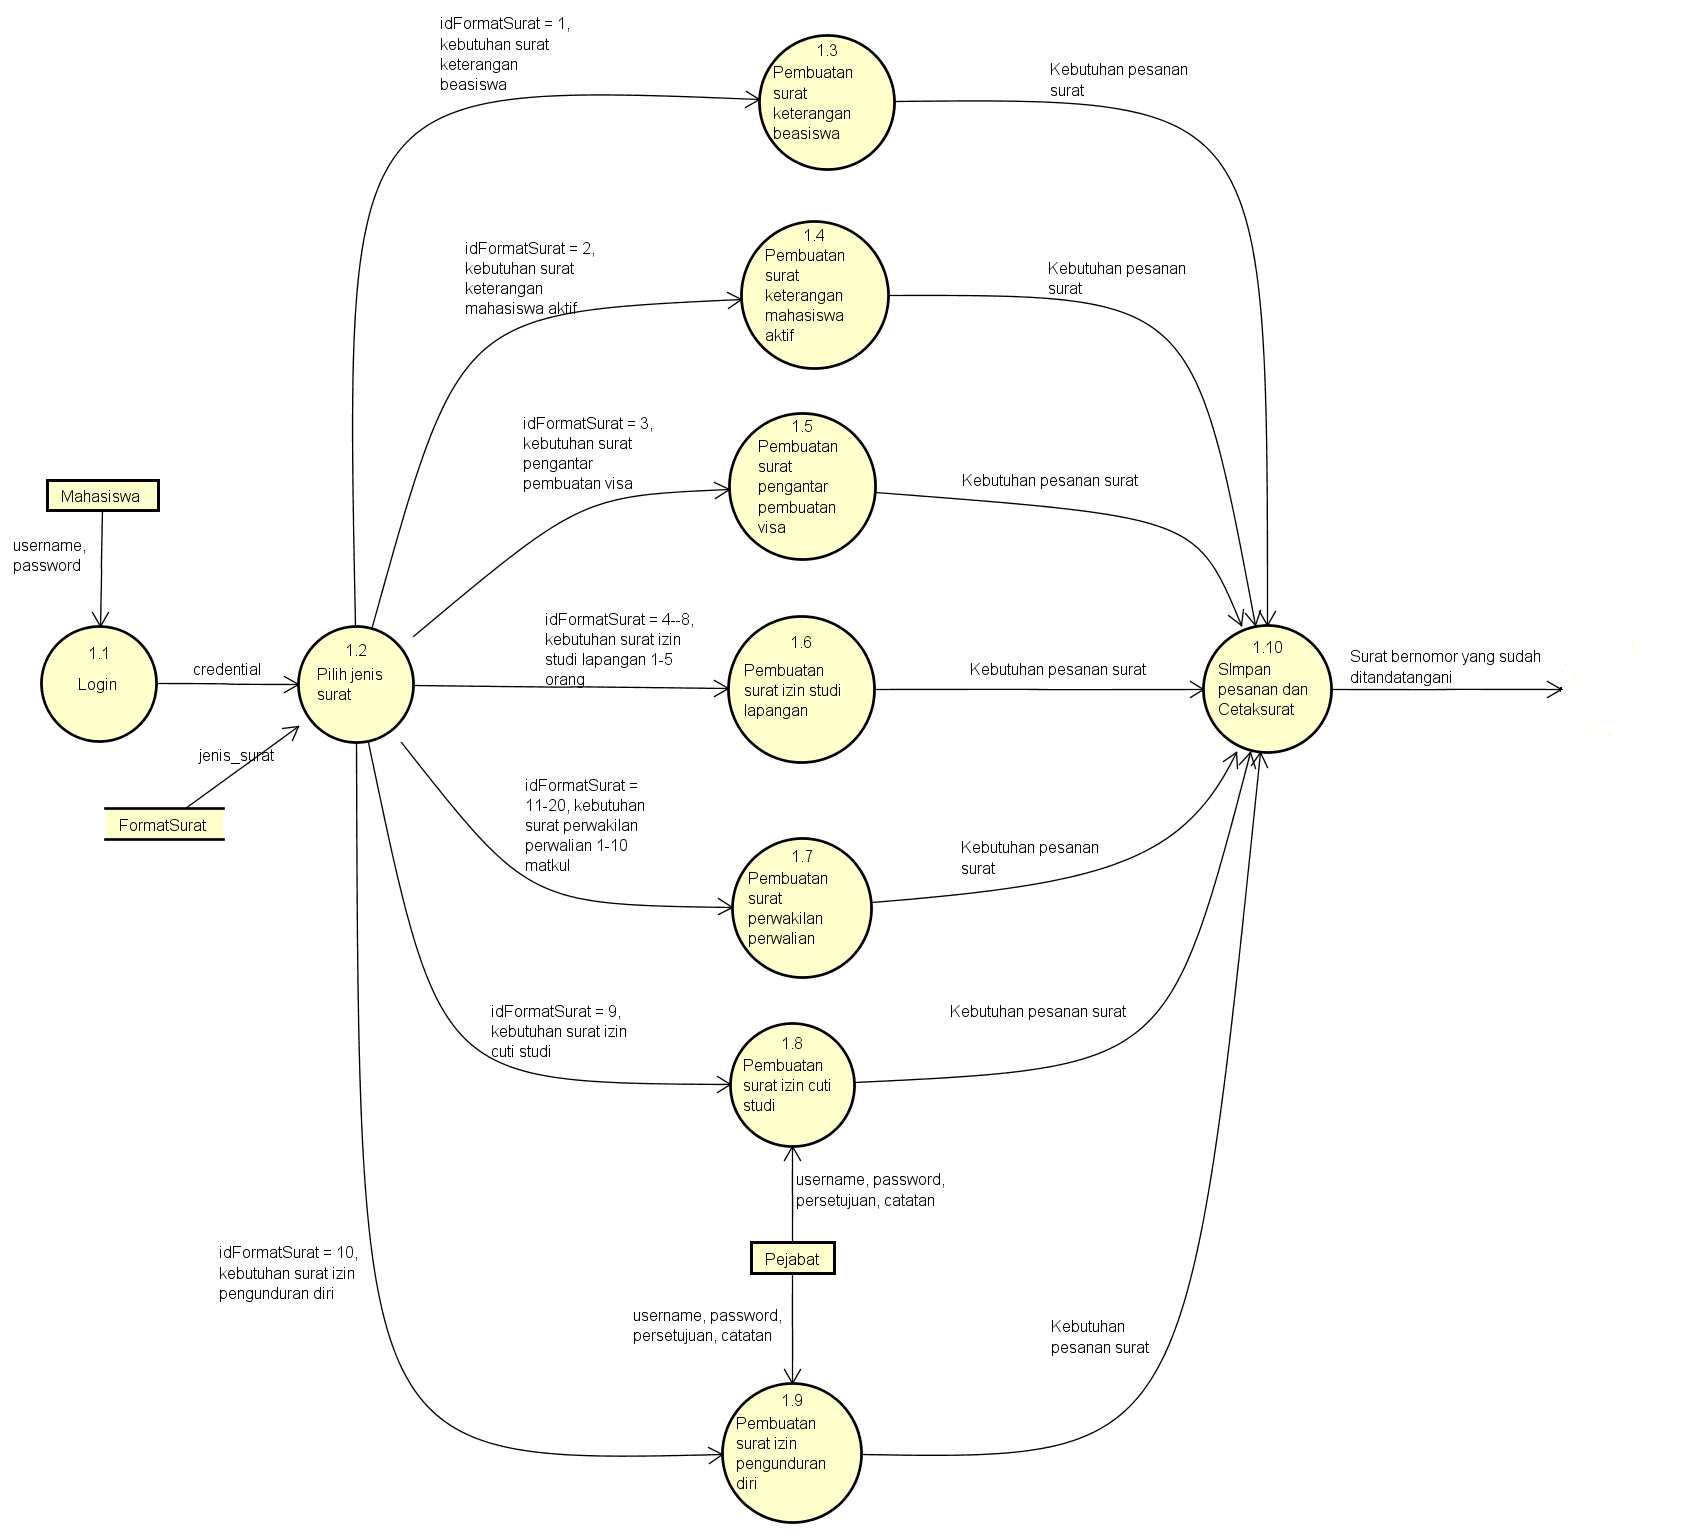
\includegraphics[scale = 0.4]{F:/Skripsi/Dokumentasi_Skripsi/Gambar/Diagram/sistem_usulan/dfd/Lv2-1_buat_suratt.png}
	\caption{DFD \textit{level} 2-1 untuk pembuatan surat}
	\label{fig:level_2-1}
\end{figure}

\begin{figure}[H]
	\centering
		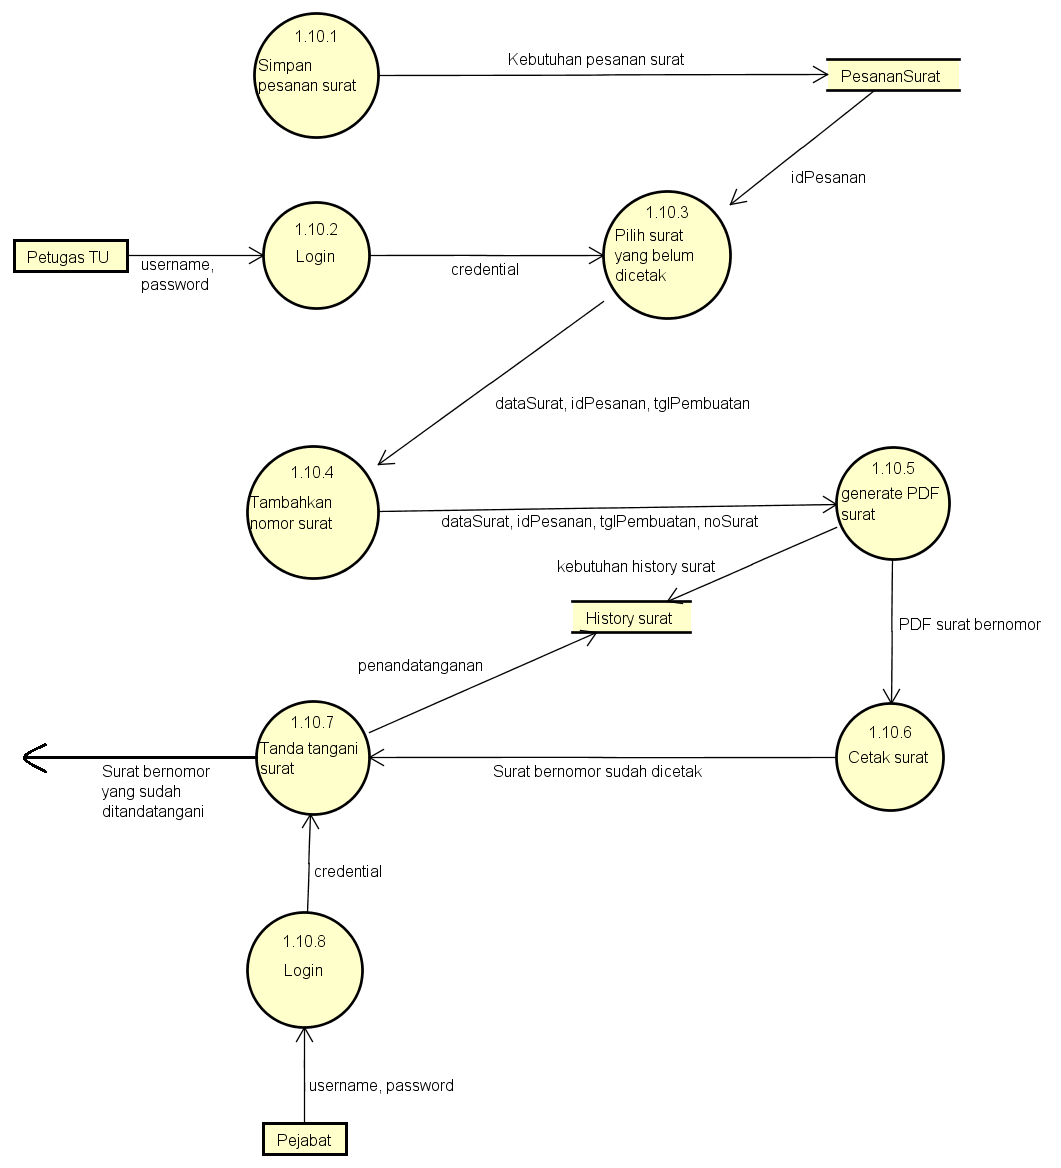
\includegraphics[scale = 0.5]{F:/Skripsi/Dokumentasi_Skripsi/Gambar/Diagram/sistem_usulan/dfd/Lv3-1_10_buat_surat_lanjutan.png}
	\caption{DFD \textit{level} 3-1.10 sebagai lanjutan untuk proses pembuatan surat}
	\label{fig:level_3-1.10}
\end{figure}

Gambar \hyperlink{level_3-1.3}{3.11} merupakan DFD \textit{level} 3-1.3 yang menjelaskan aliran data apabila aktor mahasiswa hendak membuat surat keterangan beasiswa.
\begin{figure}[H]
	\centering
		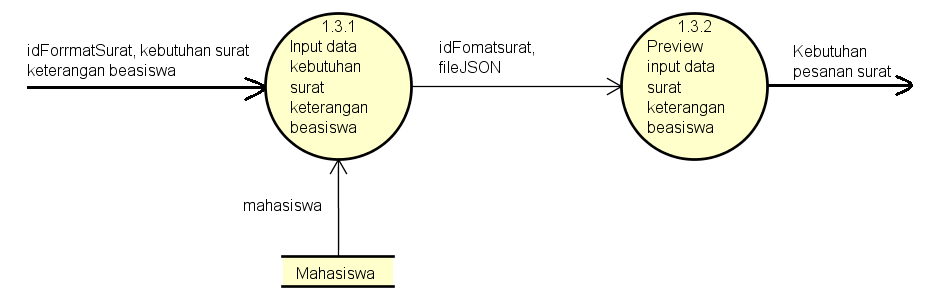
\includegraphics[scale = 0.65]{F:/Skripsi/Dokumentasi_Skripsi/Gambar/Diagram/sistem_usulan/dfd/Lv3-1_3_input_keterangan_beasiswa.png}
	\caption{DFD \textit{level} 3-1.3 untuk pembuatan surat keterangan beasiswa}
	\label{fig:level_3-1.3}
\end{figure}

Gambar \hyperlink{level_3-1.4}{3.12} merupakan DFD \textit{level} 3-1.4 yang menjelaskan aliran data apabila aktor mahasiswa hendak membuat surat keterangan mahasiswa aktif.
\begin{figure}[H]
	\centering
		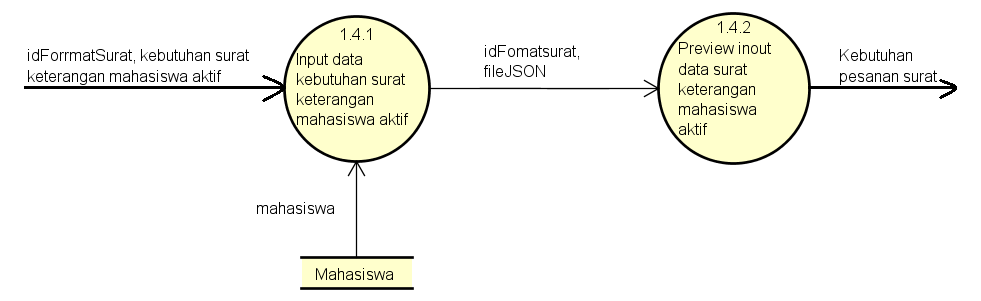
\includegraphics[scale = 0.6]{F:/Skripsi/Dokumentasi_Skripsi/Gambar/Diagram/sistem_usulan/dfd/Lv3-1_4_input_keterangan_mahasiswa_aktif.png}
	\caption{DFD \textit{level} 3-1.4 untuk pembuatan surat keterangan mahasiswa aktif}
	\label{fig:level_3-1.4}
\end{figure}

Gambar \hyperlink{level_3-1.6}{3.13} merupakan DFD \textit{level} 3-1.6 yang menjelaskan aliran data apabila aktor mahasiswa hendak membuat surat pembuatan visa.
\begin{figure}[H]
	\centering
		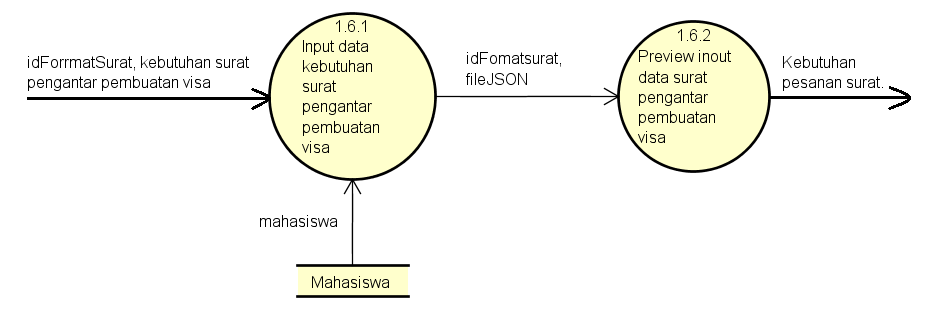
\includegraphics[scale = 0.6]{F:/Skripsi/Dokumentasi_Skripsi/Gambar/Diagram/sistem_usulan/dfd/Lv3-1_6_input_pengantar_pembuatan_visa.png}
	\caption{DFD \textit{level} 3-1.6 untuk pembuatan surat keterangan mahasiswa aktif}
	\label{fig:level_3-1.6}
\end{figure}

Gambar \hyperlink{level_3-1.5}{3.14} merupakan DFD \textit{level} 3-1.5 yang menjelaskan aliran data apabila aktor mahasiswa hendak membuat surat izin studi lapangan.
\begin{figure}[H]
	\centering
		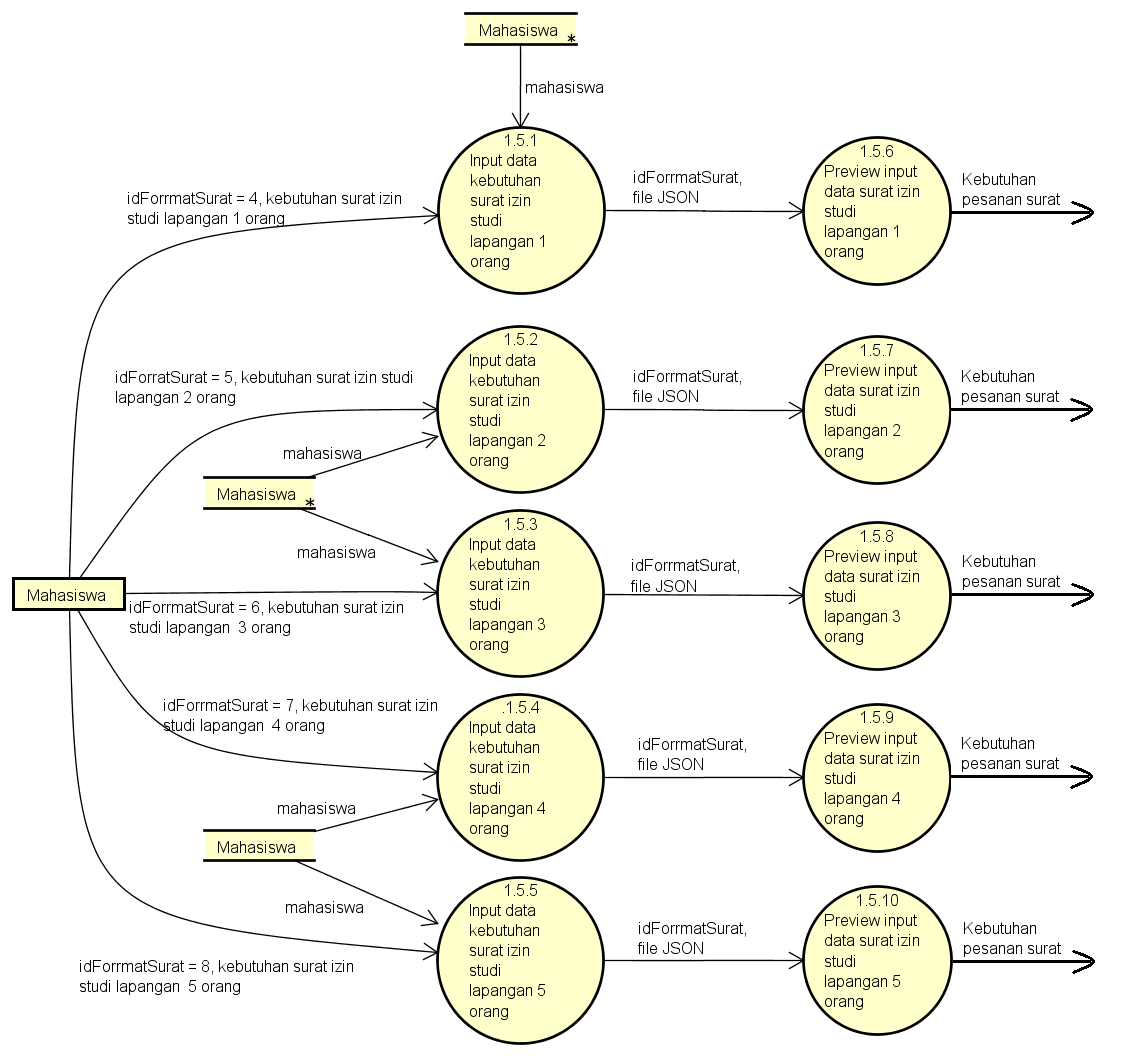
\includegraphics[scale = 0.55]{F:/Skripsi/Dokumentasi_Skripsi/Gambar/Diagram/sistem_usulan/dfd/Lv3-1_5_input_izin_studi_lapangan.png}
	\caption{DFD \textit{level} 3-1.5 untuk pembuatan surat izin studi lapangan}
	\label{fig:level_3-1.5}
\end{figure}

Gambar \hyperlink{level_3-1.7}{3.15} merupakan DFD \textit{level} 3-1.7 yang menjelaskan aliran data apabila aktor mahasiswa hendak membuat surat perwakilan perwalian.
\begin{figure}[H]
	\centering
		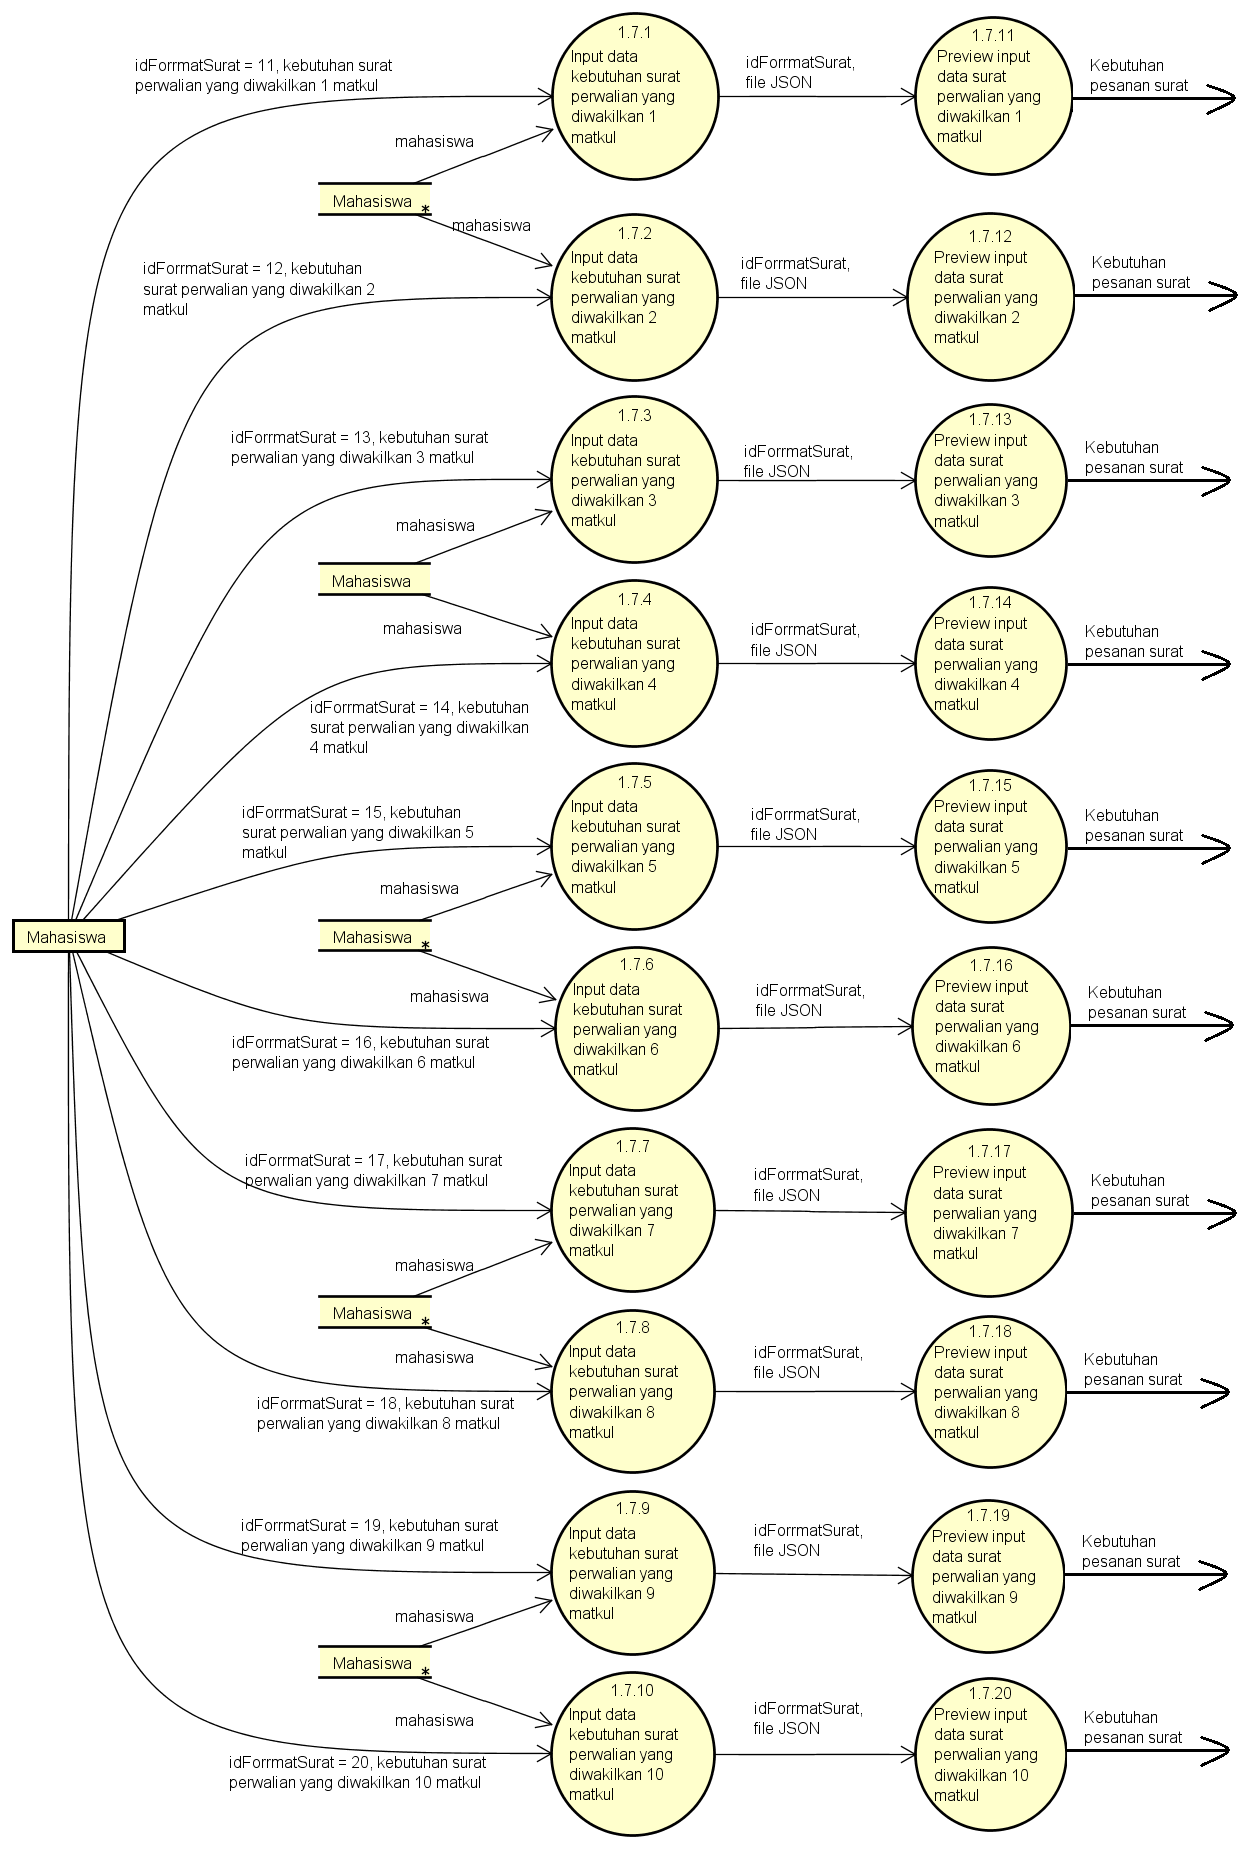
\includegraphics[scale = 0.45]{F:/Skripsi/Dokumentasi_Skripsi/Gambar/Diagram/sistem_usulan/dfd/Lv3-1_7_input_perwakilan_perwalian.png}
	\caption{DFD \textit{level} 3-1.7 untuk pembuatan surat perwakilan perwalian}
	\label{fig:level_3-1.7}
\end{figure}

Gambar \hyperlink{level_3-1.8}{3.16} merupakan DFD \textit{level} 3-1.8 yang menjelaskan aliran data apabila aktor mahasiswa hendak membuat surat izin cuti studi.
\begin{figure}[H]
	\centering
		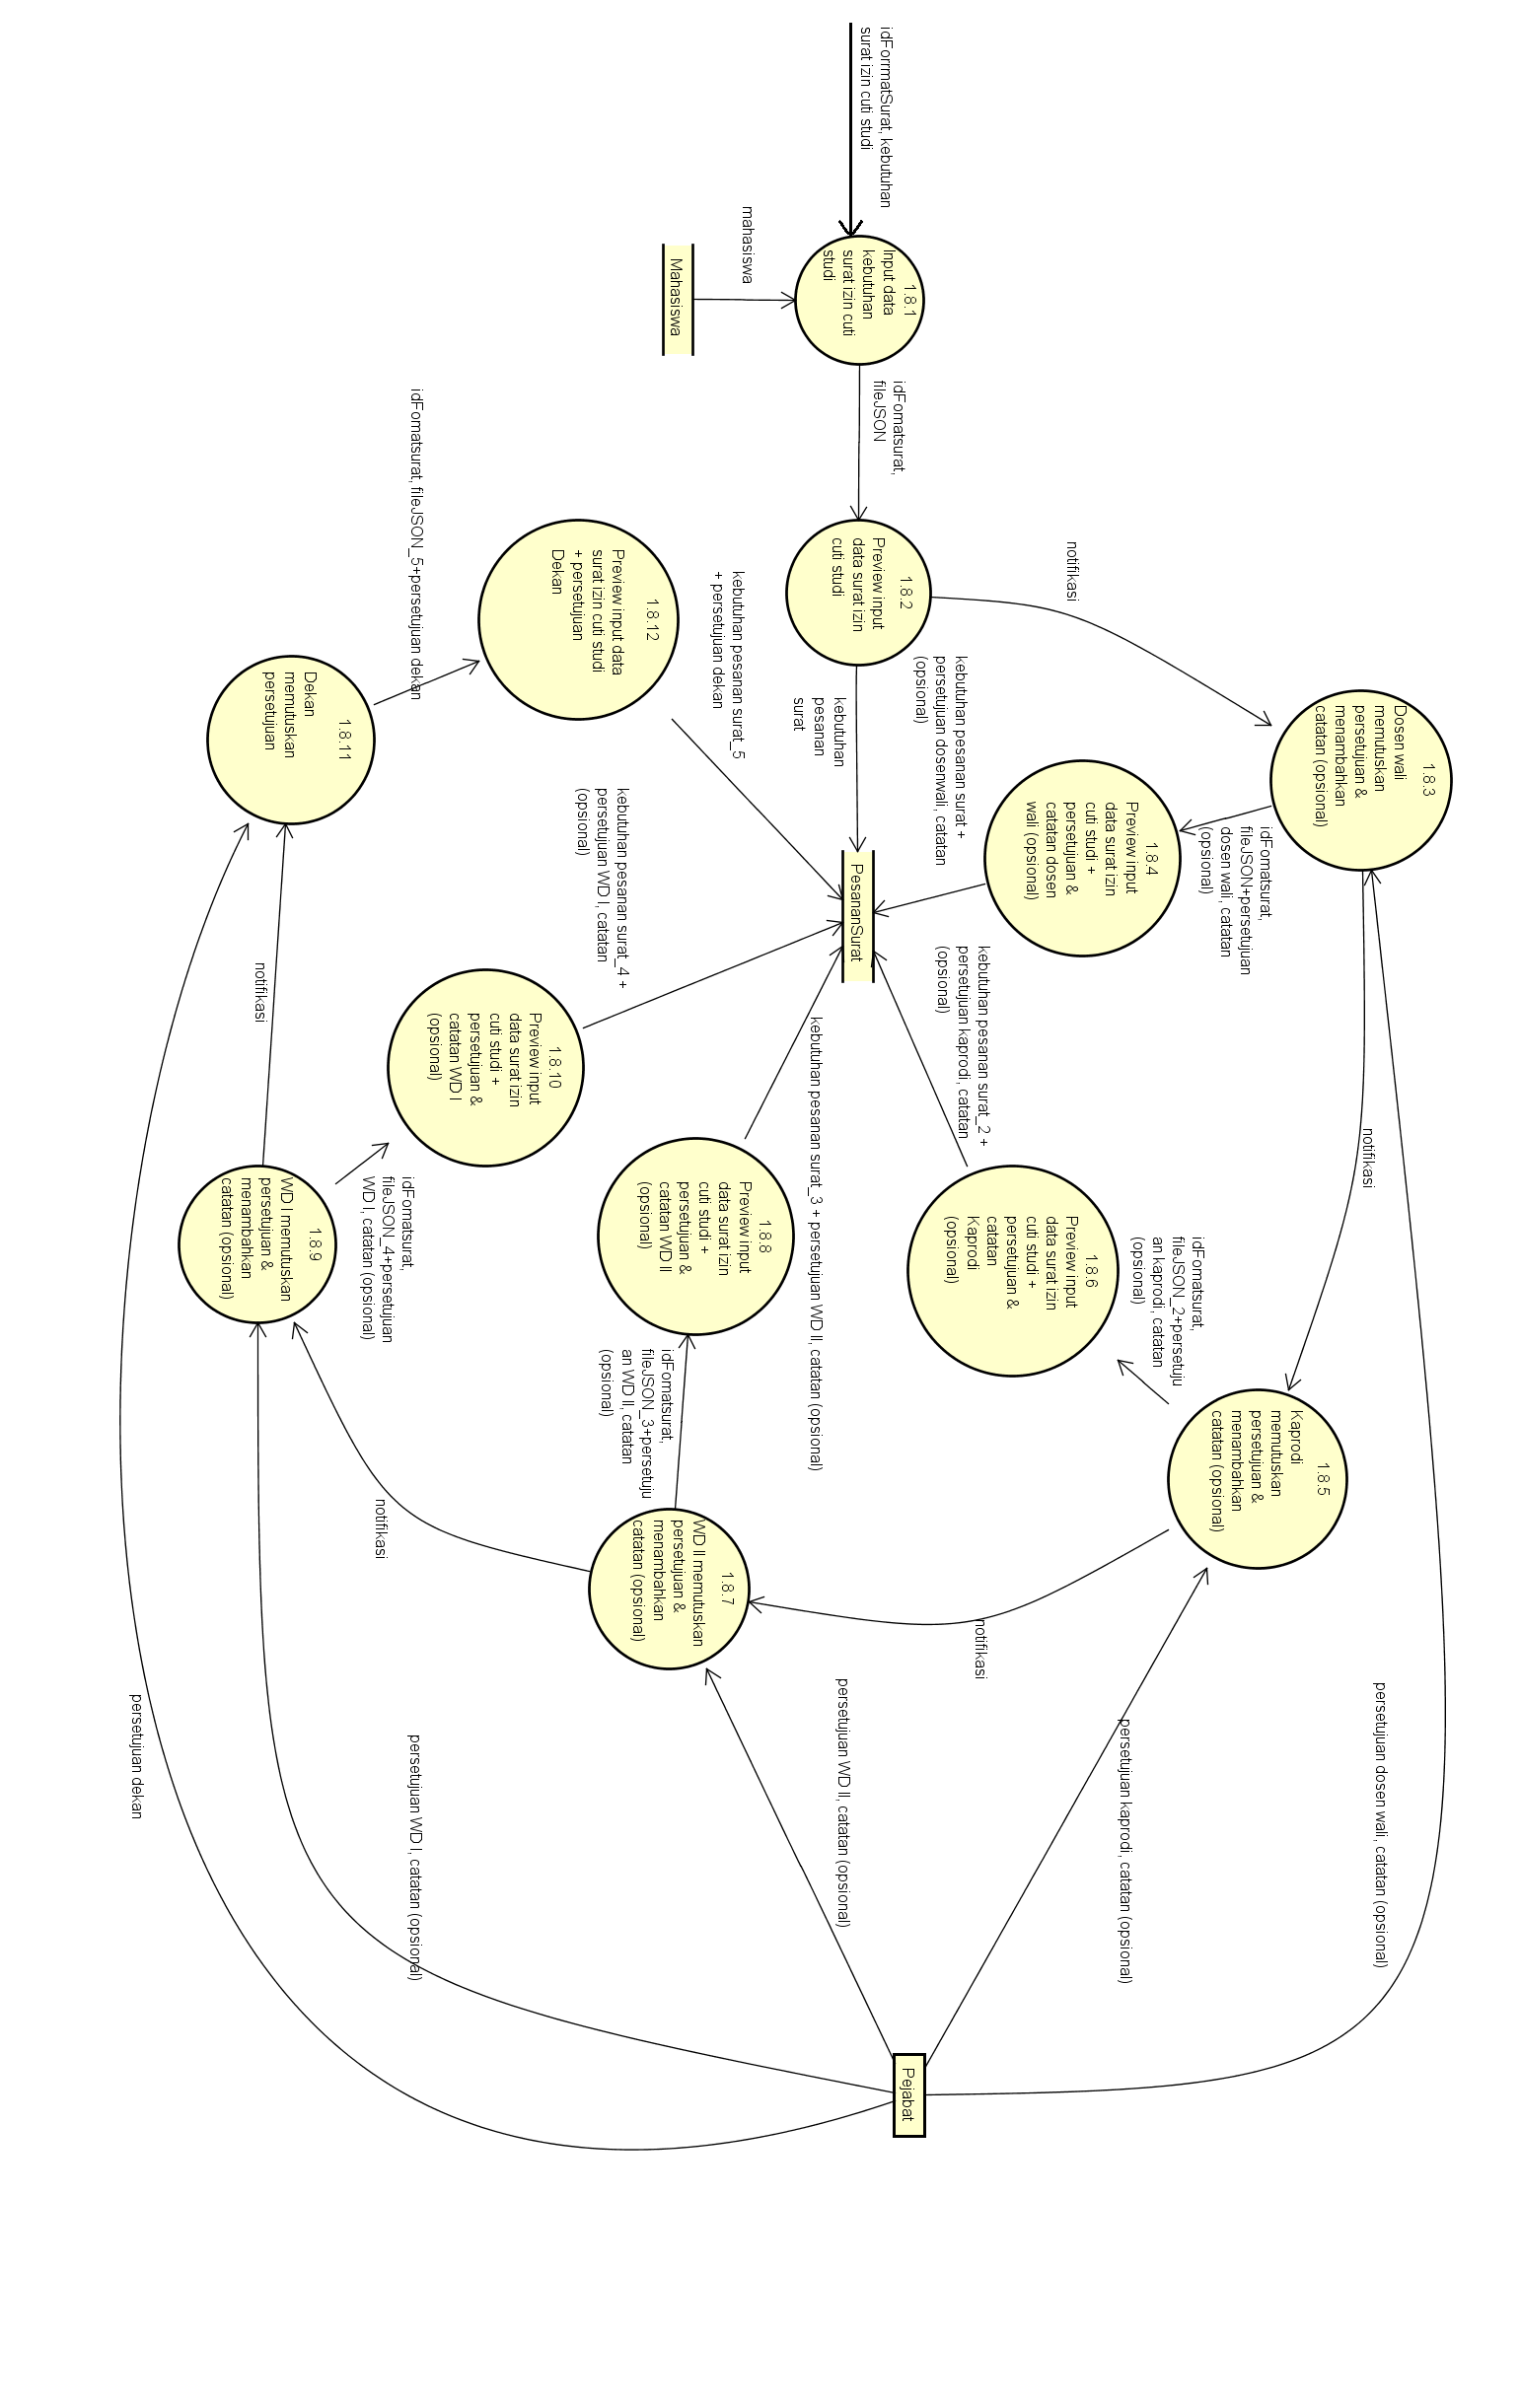
\includegraphics[scale = 0.35]{F:/Skripsi/Dokumentasi_Skripsi/Gambar/Diagram/sistem_usulan/dfd/Lv3-1_8_input_izin_cuti_studi-kiri.png}
	\caption{DFD \textit{level} 3-1.8 untuk pembuatan surat izin cuti studi}
	\label{fig:level_3-1.8}
\end{figure}

Gambar \hyperlink{level_3-1.9}{3.17} merupakan DFD \textit{level} 3-1.9 yang menjelaskan aliran data apabila aktor mahasiswa hendak membuat surat izin pengunduran diri.
\begin{figure}[H]
	\centering
		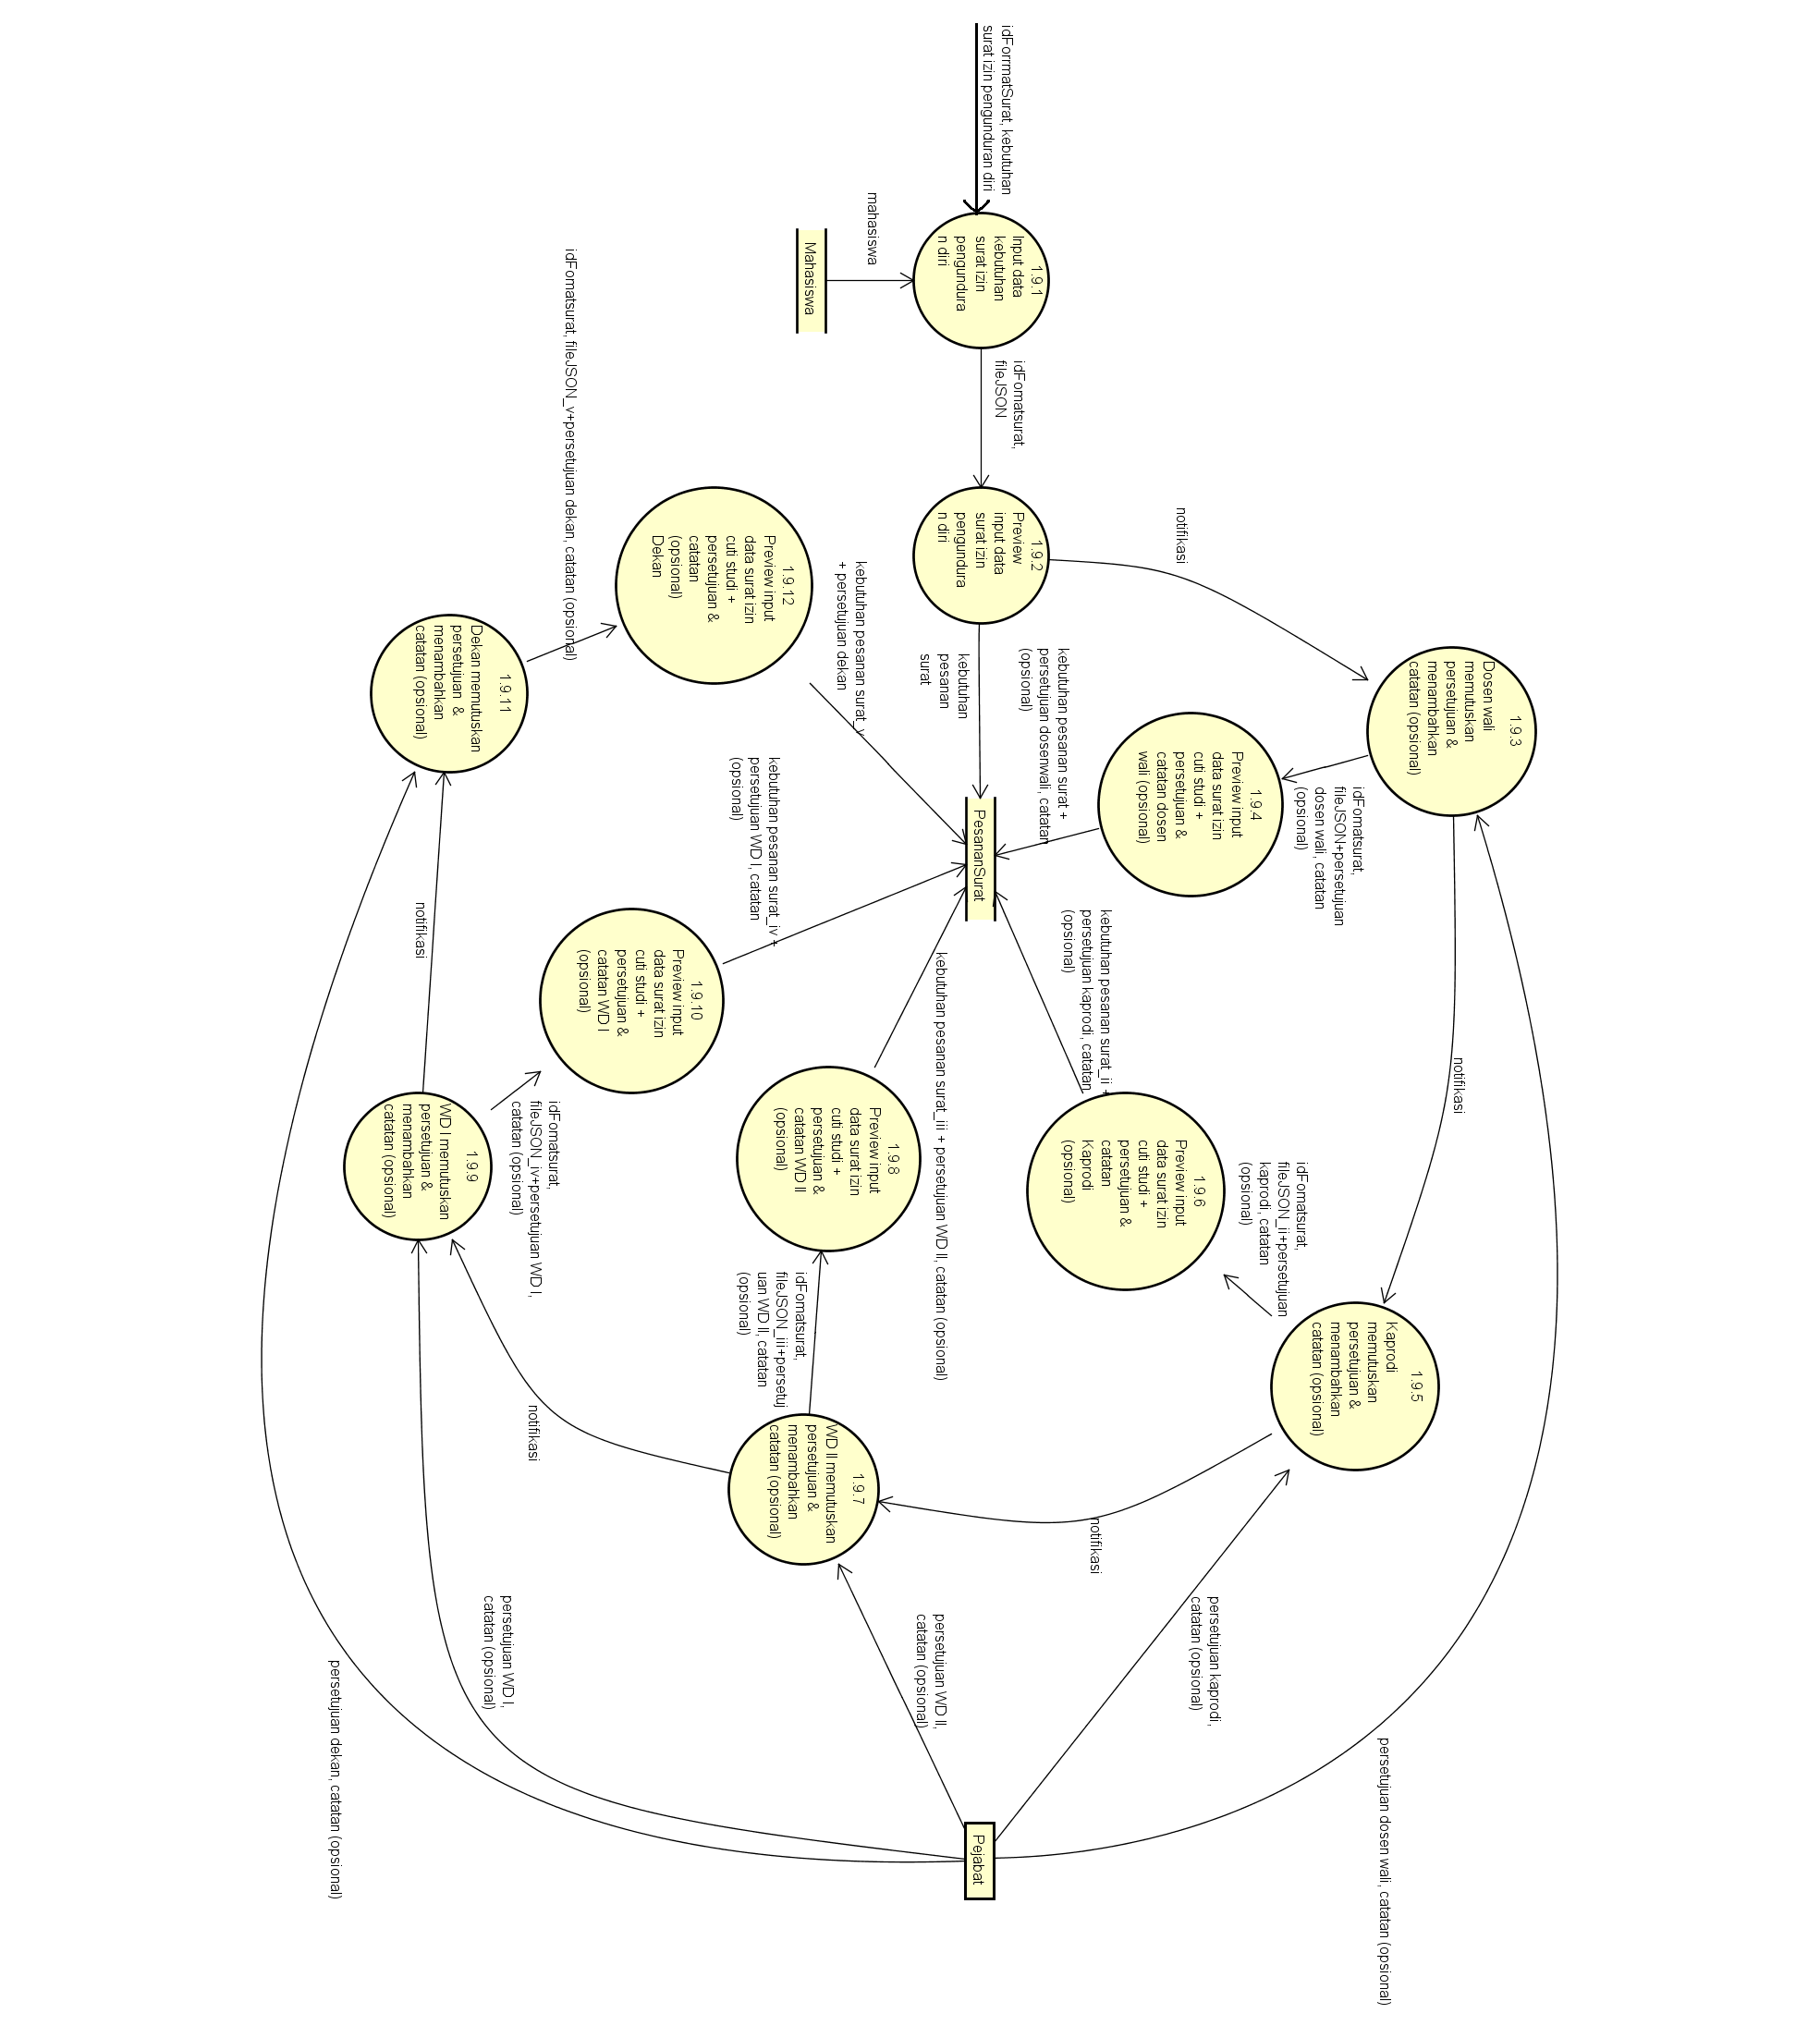
\includegraphics[scale = 0.35]{F:/Skripsi/Dokumentasi_Skripsi/Gambar/Diagram/sistem_usulan/dfd/Lv3-1_9_input_izin_pengunduran_diri-kiri.png}
	\caption{DFD \textit{level} 3-1.9 untuk pembuatan surat izin pengunduran diri}
	\label{fig:level_3-1.9}
\end{figure}

Gambar \hyperlink{level_2-2}{3.18} merupakan DFD \textit{level} 2-2 yang menjelaskan aliran data pada saat aktor mahasiswa hendak mengambil surat.

\begin{figure}[H]
	\centering
		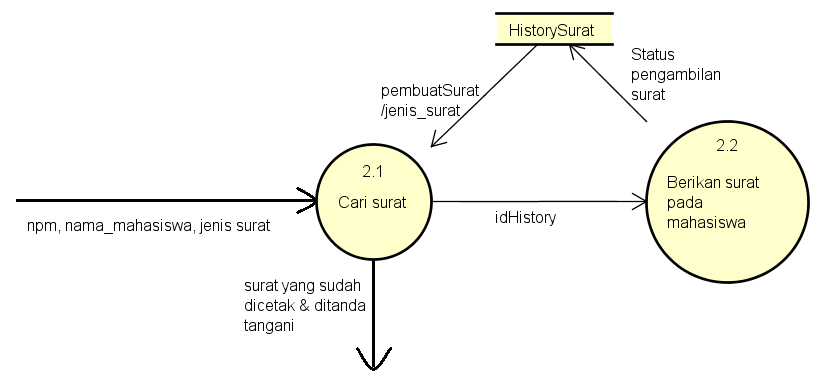
\includegraphics[scale = 0.5]{F:/Skripsi/Dokumentasi_Skripsi/Gambar/Diagram/sistem_usulan/dfd/Lv2-2_pengambilan_surat.png}
	\caption{DFD \textit{level} 2-2 pengambilan surat}
	\label{fig:level_2-2}
\end{figure}

Gambar \hyperlink{level_2-3}{3.19} merupakan DFD \textit{level} 2-3 yang menjelaskan aliran data pada saat aktor petugas TU melakukan operasi CRUD pada \textit{database} format surat.

\begin{figure}[H]
	\centering
		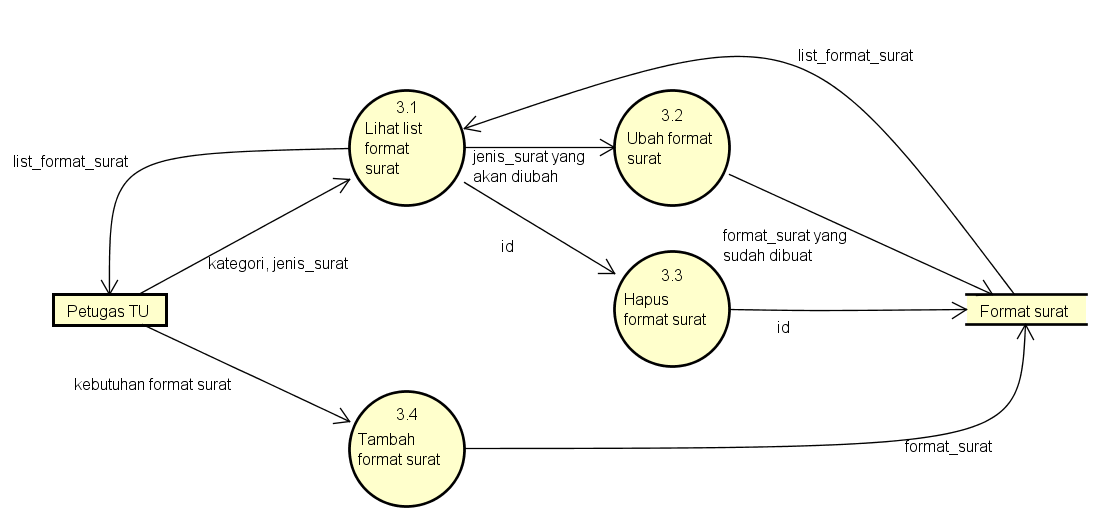
\includegraphics[scale = 0.5]{F:/Skripsi/Dokumentasi_Skripsi/Gambar/Diagram/sistem_usulan/dfd/Lv2-3_kelola_format_surat.png}
	\caption{DFD \textit{level} 2-3 operasi CRUD pada \textit{database} format surat}
	\label{fig:level_2-3}
\end{figure}

Gambar \hyperlink{level_2-4}{3.20} merupakan DFD \textit{level} 2-4 yang menjelaskan aliran data pada saat aktor petugas TU melakukan operasi CRUD pada \textit{database} data mahasiswa.

\begin{figure}[H]
	\centering
		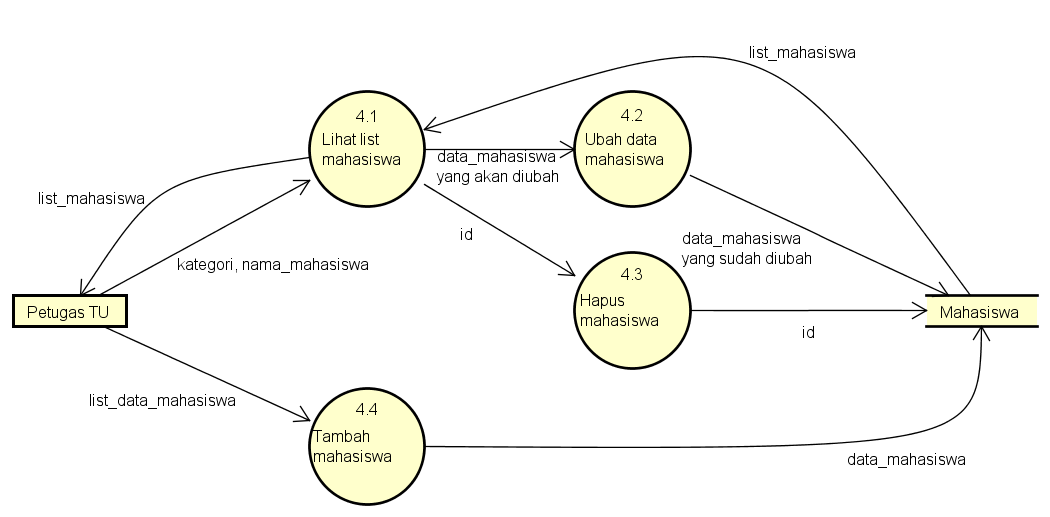
\includegraphics[scale = 0.5]{F:/Skripsi/Dokumentasi_Skripsi/Gambar/Diagram/sistem_usulan/dfd/Lv2-4_kelola_data_mahasiswa.png}
	\caption{DFD \textit{level} 2-4 operasi CRUD pada \textit{database} data mahasiswa}
	\label{fig:level_2-4}
\end{figure}

\textbf{Data Dictionary}\\
\begin{itemize}
 \item list data mahaiswa : nirm, npm, nama mahasiswa, prodi, fakultas, angkatan, tglLahir, kota lahir, foto, dosenWali, username, password
 \item data per mahasiswa : nirm, npm, nama mahasiswa, prodi, fakultas, angkatan, tglLahir, kota lahir, foto, dosenWali
 \item kebutuhan format surat : idFormat, jenis surat, format, keterangan
 \item kebutuhan pesanan surat : tglPembuatan, perihal, npm, idFormatSurat, dataSurat, penerimaSurat
 \item kebutuhan history surat : status penandatanganan surat, Status pengambilan surat
\end{itemize}

\subsection{Analisis Kebutuhan Data}
\label{sec:analisis_kebutuhan_data}
Setiap surat memiliki kebutuhan data yang berbeda-beda bergantung dari jenis surat yang akan dibuat. Tabel 3.16-3.20 berikut ini akan menjelaskan data apa saja yang perlu diisikan oleh mahasiswa dalam proses pembuatan surat akademik.\

\begin{table}[h]
\centering
\caption{Tabel kebutuhan data surat keterangan beasiswa}
\label{surat_keterangan_beasiswa}
\begin{tabular}{|l|}
\hline
\textbf{Atribut Data}                     \\ \hline
Nama mahasiswa                            \\ \hline 
Program studi                             \\ \hline 
NPM                             			\\ \hline
Semester			                        \\ \hline
Tahun akademik        			        \\ \hline
Penyedia beasiswa                         \\ \hline
\end{tabular}
\end{table}

\begin{table}[h]
\centering
\caption{Tabel kebutuhan data surat keterangan mahasiswa aktif}
\label{surat_keterangan_mahasiswa_aktif}
\begin{tabular}{|l|}
\hline
\textbf{Atribut Data}                     \\ \hline
Nama mahasiswa                            \\ \hline 
Program studi                             \\ \hline 
NPM                             			\\ \hline 
Semester                     				\\ \hline 
Tahun akademik                         	\\ \hline 
Kota lahir               					\\ \hline 
Tanggal lahir             				\\ \hline 
Alamat di Bandung                    		\\ \hline 
\end{tabular}
\end{table}

\begin{table}[h]
\centering
\caption{Tabel kebutuhan data surat pengantar pembuatan visa}
\label{surat_pengantar_pembuatan_visa}
\begin{tabular}{|l|}
\hline
\textbf{Atribut Data}                     \\ \hline
Nama mahasiswa                            \\ \hline 
Tanggal lahir                    			\\ \hline 
Kewarganegaraan                     	    \\ \hline 
Tahun akademik              				\\ \hline 
Organisasi tujuan         			    \\ \hline 
Negara tujuan              			    \\ \hline 
Tanggal kunjungan                         \\ \hline 
\end{tabular}
\end{table}

\begin{table}[h]
\centering
\caption{Tabel kebutuhan data surat pengantar studi lapangan}
\label{surat_keterangan_beasiswa}
\begin{tabular}{|l|}
\hline
\textbf{Atribut Data}                     \\ \hline
Nama mahasiswa                            \\ \hline 
NPM                                      \\ \hline 
Program studi                             \\ \hline
Mata kuliah			                    \\ \hline
Topik        			                    \\ \hline
Organisasi tujuan                         \\ \hline
Alamat organisasi tujuan                  \\ \hline
Keperluan kunjungan                       \\ \hline
Data rekan(nama, NPM rekan)(opsional)     \\ \hline

\end{tabular}
\end{table}

\begin{table}[H]
\centering
\caption{Tabel kebutuhan data surat izin cuti studi}
\label{surat_izin_cuti_studi}
\begin{tabular}{|l|}
\hline
{\textbf{Atribut Data}}                     \\ \hline
Nama mahasiswa                            \\ \hline 
NPM                                       \\ \hline 
Fakultas                                  \\ \hline 
Program studi                             \\ \hline 
Alamat tetap                              \\ \hline
Cuti studi ke-n   			            \\ \hline 
Alasan cuti studi ke-n                    \\ \hline
Dosen Wali				                \\ \hline 
Catatan Dosen Wali                        \\ \hline
Catatan Ketua Progam Studi                \\ \hline 
Rekomendasi Pembantu Dekan II             \\ \hline 
Rekomendasi Pembantu Dekan I              \\ \hline 
Semester                          		\\ \hline 
Tahun akademik                            \\ \hline
Persetujuan Dekan                         \\ \hline 
Tanggal surat                             \\ \hline
\end{tabular}
\end{table}

\begin{table}[H]
\centering
\caption{Tabel kebutuhan data surat izin pengunduran diri}
\label{surat_izin_pengunduran_diri}
\begin{tabular}{|l|}
\hline
\textbf{Atribut Data}                     \\ \hline
Nama mahasiswa                            \\ \hline 
NPM                                       \\ \hline 
NIRM                                      \\ \hline 
Alamat (tetap/di Badung)                  \\ \hline 
Nomor telepon (HP)                        \\ \hline 
Nama orang tua                            \\ \hline 
Tanggal surat                             \\ \hline 
Semester berhenti                         \\ \hline 
Catatan Dosen Wali                        \\ \hline 
Catatan Ketua Program Studi               \\ \hline 
Catatan Wakil Dekan I                     \\ \hline 
Catatan Wakil Dekan II                    \\ \hline 
Catatan Dekan                             \\ \hline
\end{tabular}
\end{table}

\begin{table}[H]
\centering
\caption{Tabel kebutuhan data surat perwakilan perwalian}
\label{surat_perwakilan_perwalian}
\begin{tabular}{|l|}
\hline
\textbf{Atribut Data}                      \\ \hline
Semester            					   \\ \hline
Tahun akademik							   \\ \hline
Nama mahasiswa yang diwakilkan             \\ \hline 
NPM mahasiswa yang diwakilkan              \\ \hline 
Program Studi mahasiswa yang diwakilkan    \\ \hline 
Nama mahasiswa yang diberi kuasa           \\ \hline 
NPM mahasiswa yang diberi kuasa            \\ \hline 
Program studi mahasiswa yang diberi kuasa  \\ \hline 
Alasan tidak hadir perwalian               \\ \hline 
Mata kuliah yang diambil (maks. 10 mata kuliah)                  \\ \hline 
Tanggal pembuatan surat                    \\ \hline
Nama dosen wali							   \\ \hline
Nama wakil dekan I						   \\ \hline
\end{tabular}
\end{table}

\subsection{ER Diagram}
\label{sec:er_diagram}
Setelah mengamati \textit{work flowmap}, didapat beberapa objek yang dapat digambarkan menjadi sebuah entitas pada diagram ER. Objek-objek yang dimaksud yaitu format surat, mahasiswa, petugas TU dan pejabat. Untuk objek surat dan mahasiswa dapat langsung dibuat entitas. Untuk objek pejabat diubah menjadi entitas dosen karena pejabat merupakan dosen yang memiliki pangkat tertentu di jurusan maupun fakultas.\

Selain objek yang didapat dari \textit{work flowmap}, didapat juga objek-objek lain yang berhubungan dengan objek-objek yang telah disebutkan. Objek-objek yang dimaksud yaitu jurusan, fakultas, pesanan surat dan \textit{history} surat. Gambar \hyperlink{erd}{3.21} adalah diagram ER yang menggambarkan hubungan antar entitas yang telah disebutkan di atas.

\begin{figure}[H]
	\centering
		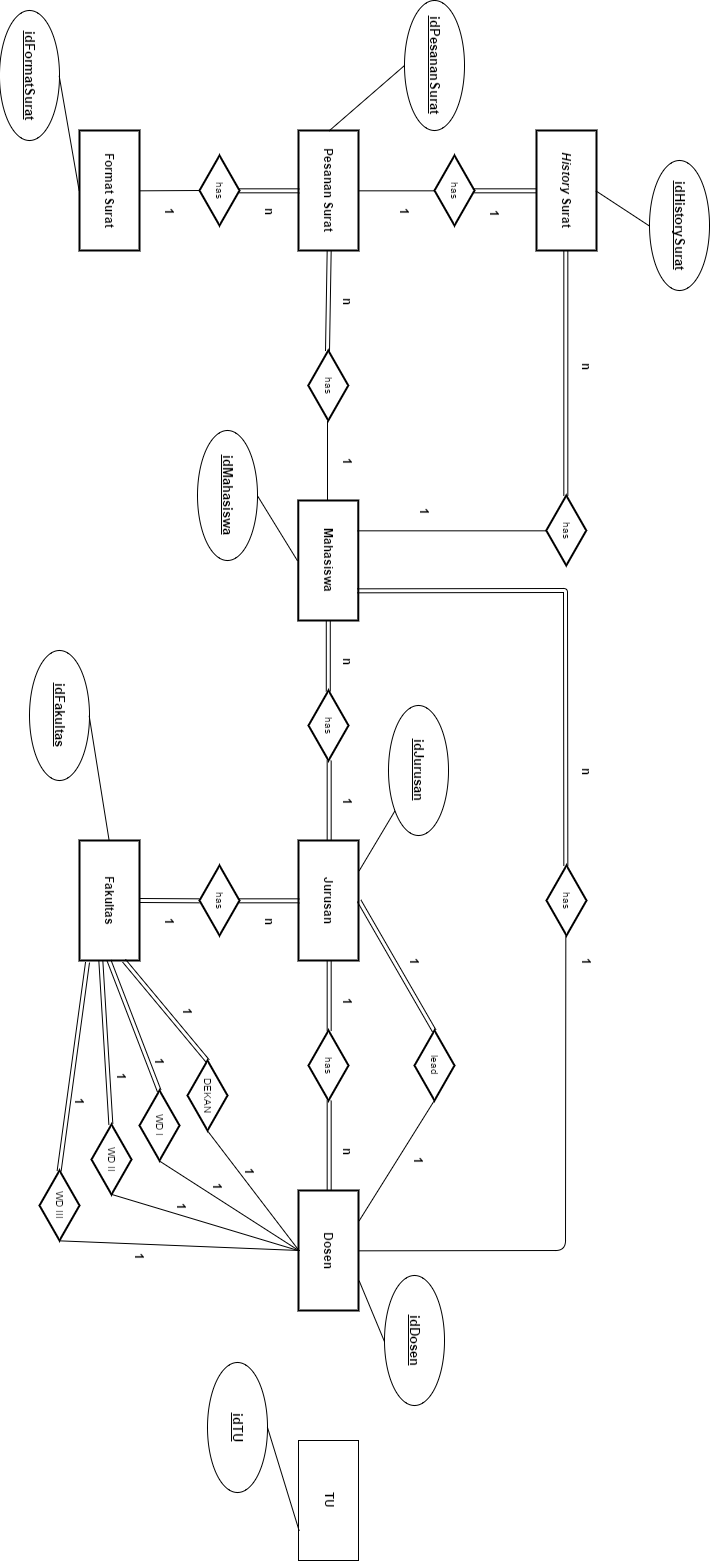
\includegraphics[scale = 0.5]{F:/Skripsi/Dokumentasi_Skripsi/Gambar/Diagram/sistem_usulan/erd/erd_left.png}
	\caption{Diagram ER}
	\label{fig:level_2-2}
\end{figure}